\documentclass[]{article}
\usepackage{lmodern}
\usepackage{amssymb,amsmath}
\usepackage{ifxetex,ifluatex}
\usepackage{fixltx2e} % provides \textsubscript
\ifnum 0\ifxetex 1\fi\ifluatex 1\fi=0 % if pdftex
  \usepackage[T1]{fontenc}
  \usepackage[utf8]{inputenc}
\else % if luatex or xelatex
  \ifxetex
    \usepackage{mathspec}
  \else
    \usepackage{fontspec}
  \fi
  \defaultfontfeatures{Ligatures=TeX,Scale=MatchLowercase}
\fi
% use upquote if available, for straight quotes in verbatim environments
\IfFileExists{upquote.sty}{\usepackage{upquote}}{}
% use microtype if available
\IfFileExists{microtype.sty}{%
\usepackage{microtype}
\UseMicrotypeSet[protrusion]{basicmath} % disable protrusion for tt fonts
}{}
\usepackage[margin=1in]{geometry}
\usepackage{hyperref}
\hypersetup{unicode=true,
            pdftitle={rtapas: An R Package to Implement Thresholding Approach for Probability Map Automatic Segmentation (TAPAS)},
            pdfauthor={Alessandra Valcarcel},
            pdfborder={0 0 0},
            breaklinks=true}
\urlstyle{same}  % don't use monospace font for urls
\usepackage{color}
\usepackage{fancyvrb}
\newcommand{\VerbBar}{|}
\newcommand{\VERB}{\Verb[commandchars=\\\{\}]}
\DefineVerbatimEnvironment{Highlighting}{Verbatim}{commandchars=\\\{\}}
% Add ',fontsize=\small' for more characters per line
\usepackage{framed}
\definecolor{shadecolor}{RGB}{248,248,248}
\newenvironment{Shaded}{\begin{snugshade}}{\end{snugshade}}
\newcommand{\AlertTok}[1]{\textcolor[rgb]{0.94,0.16,0.16}{#1}}
\newcommand{\AnnotationTok}[1]{\textcolor[rgb]{0.56,0.35,0.01}{\textbf{\textit{#1}}}}
\newcommand{\AttributeTok}[1]{\textcolor[rgb]{0.77,0.63,0.00}{#1}}
\newcommand{\BaseNTok}[1]{\textcolor[rgb]{0.00,0.00,0.81}{#1}}
\newcommand{\BuiltInTok}[1]{#1}
\newcommand{\CharTok}[1]{\textcolor[rgb]{0.31,0.60,0.02}{#1}}
\newcommand{\CommentTok}[1]{\textcolor[rgb]{0.56,0.35,0.01}{\textit{#1}}}
\newcommand{\CommentVarTok}[1]{\textcolor[rgb]{0.56,0.35,0.01}{\textbf{\textit{#1}}}}
\newcommand{\ConstantTok}[1]{\textcolor[rgb]{0.00,0.00,0.00}{#1}}
\newcommand{\ControlFlowTok}[1]{\textcolor[rgb]{0.13,0.29,0.53}{\textbf{#1}}}
\newcommand{\DataTypeTok}[1]{\textcolor[rgb]{0.13,0.29,0.53}{#1}}
\newcommand{\DecValTok}[1]{\textcolor[rgb]{0.00,0.00,0.81}{#1}}
\newcommand{\DocumentationTok}[1]{\textcolor[rgb]{0.56,0.35,0.01}{\textbf{\textit{#1}}}}
\newcommand{\ErrorTok}[1]{\textcolor[rgb]{0.64,0.00,0.00}{\textbf{#1}}}
\newcommand{\ExtensionTok}[1]{#1}
\newcommand{\FloatTok}[1]{\textcolor[rgb]{0.00,0.00,0.81}{#1}}
\newcommand{\FunctionTok}[1]{\textcolor[rgb]{0.00,0.00,0.00}{#1}}
\newcommand{\ImportTok}[1]{#1}
\newcommand{\InformationTok}[1]{\textcolor[rgb]{0.56,0.35,0.01}{\textbf{\textit{#1}}}}
\newcommand{\KeywordTok}[1]{\textcolor[rgb]{0.13,0.29,0.53}{\textbf{#1}}}
\newcommand{\NormalTok}[1]{#1}
\newcommand{\OperatorTok}[1]{\textcolor[rgb]{0.81,0.36,0.00}{\textbf{#1}}}
\newcommand{\OtherTok}[1]{\textcolor[rgb]{0.56,0.35,0.01}{#1}}
\newcommand{\PreprocessorTok}[1]{\textcolor[rgb]{0.56,0.35,0.01}{\textit{#1}}}
\newcommand{\RegionMarkerTok}[1]{#1}
\newcommand{\SpecialCharTok}[1]{\textcolor[rgb]{0.00,0.00,0.00}{#1}}
\newcommand{\SpecialStringTok}[1]{\textcolor[rgb]{0.31,0.60,0.02}{#1}}
\newcommand{\StringTok}[1]{\textcolor[rgb]{0.31,0.60,0.02}{#1}}
\newcommand{\VariableTok}[1]{\textcolor[rgb]{0.00,0.00,0.00}{#1}}
\newcommand{\VerbatimStringTok}[1]{\textcolor[rgb]{0.31,0.60,0.02}{#1}}
\newcommand{\WarningTok}[1]{\textcolor[rgb]{0.56,0.35,0.01}{\textbf{\textit{#1}}}}
\usepackage{graphicx,grffile}
\makeatletter
\def\maxwidth{\ifdim\Gin@nat@width>\linewidth\linewidth\else\Gin@nat@width\fi}
\def\maxheight{\ifdim\Gin@nat@height>\textheight\textheight\else\Gin@nat@height\fi}
\makeatother
% Scale images if necessary, so that they will not overflow the page
% margins by default, and it is still possible to overwrite the defaults
% using explicit options in \includegraphics[width, height, ...]{}
\setkeys{Gin}{width=\maxwidth,height=\maxheight,keepaspectratio}
\IfFileExists{parskip.sty}{%
\usepackage{parskip}
}{% else
\setlength{\parindent}{0pt}
\setlength{\parskip}{6pt plus 2pt minus 1pt}
}
\setlength{\emergencystretch}{3em}  % prevent overfull lines
\providecommand{\tightlist}{%
  \setlength{\itemsep}{0pt}\setlength{\parskip}{0pt}}
\setcounter{secnumdepth}{0}
% Redefines (sub)paragraphs to behave more like sections
\ifx\paragraph\undefined\else
\let\oldparagraph\paragraph
\renewcommand{\paragraph}[1]{\oldparagraph{#1}\mbox{}}
\fi
\ifx\subparagraph\undefined\else
\let\oldsubparagraph\subparagraph
\renewcommand{\subparagraph}[1]{\oldsubparagraph{#1}\mbox{}}
\fi

%%% Use protect on footnotes to avoid problems with footnotes in titles
\let\rmarkdownfootnote\footnote%
\def\footnote{\protect\rmarkdownfootnote}

%%% Change title format to be more compact
\usepackage{titling}

% Create subtitle command for use in maketitle
\newcommand{\subtitle}[1]{
  \posttitle{
    \begin{center}\large#1\end{center}
    }
}

\setlength{\droptitle}{-2em}

  \title{rtapas: An R Package to Implement Thresholding Approach for Probability
Map Automatic Segmentation (TAPAS)}
    \pretitle{\vspace{\droptitle}\centering\huge}
  \posttitle{\par}
    \author{Alessandra Valcarcel}
    \preauthor{\centering\large\emph}
  \postauthor{\par}
      \predate{\centering\large\emph}
  \postdate{\par}
    \date{2019-03-12}


\begin{document}
\maketitle

\hypertarget{overview}{%
\section{Overview }\label{overview}}

The \texttt{rtapas} package determines a subject-specific threshold to
apply to multiple sclerosis lesion probability maps for automatic
segmentation. This R package is based on the Thresholding Approach for
Probability Map Automatic Segmentation (TAPAS) method. The methods are
in progress for publication. This package creates the data structures
necessary for training the TAPAS model. After training, the model can be
used to predict subject-specific thresholds to use on probability maps
for automatic lesion segmentation. Methods can be extended outside of
multiple sclerosis lesion segmentation but have not been validated.

\hypertarget{installation}{%
\section{Installation}\label{installation}}

To get the latest development version from GitHub:

\begin{Shaded}
\begin{Highlighting}[]
\CommentTok{# install.packages("remotes")}
\KeywordTok{library}\NormalTok{(remotes)}
\NormalTok{remotes}\OperatorTok{::}\KeywordTok{install_github}\NormalTok{(}\StringTok{'avalcarcel9/rtapas'}\NormalTok{)}
\end{Highlighting}
\end{Shaded}

We are currently working to get the package on
\href{www.neuroconductor.org}{Neuroconductor}.

\hypertarget{function-documentation}{%
\section{Function Documentation}\label{function-documentation}}

The TAPAS package contains a number of functions to generate data
required for training, train the model, and predict subject-specific
thresholds based on the trained model. The functions, defaults, and
usage are provided below.

\hypertarget{tapas_data}{%
\subsection{\texorpdfstring{\texttt{tapas\_data}}{tapas\_data}}\label{tapas_data}}

\begin{Shaded}
\begin{Highlighting}[]
\KeywordTok{tapas_data}\NormalTok{(}\DataTypeTok{thresholds =} \KeywordTok{seq}\NormalTok{(}\DataTypeTok{from =} \DecValTok{0}\NormalTok{, }\DataTypeTok{to =} \DecValTok{1}\NormalTok{, }\DataTypeTok{by =} \FloatTok{0.01}\NormalTok{),}
\NormalTok{           pmap,}
\NormalTok{           gold_standard,}
\NormalTok{           mask,}
           \DataTypeTok{k =} \DecValTok{8}\NormalTok{,}
           \DataTypeTok{subject_id =} \OtherTok{NULL}\NormalTok{,}
           \DataTypeTok{verbose =} \OtherTok{TRUE}\NormalTok{)}
\end{Highlighting}
\end{Shaded}

\textbf{Description}:

This function creates the training vectors for a single subject from a
probability map, a gold standard mask (normally a manual segmentation),
and a brain mask. For a grid of thresholds provided and applied to the
probability map the function calculates Sørensen's--Dice coefficient
(DSC) between the automatic image and the gold standard image. The
function also calculates the volume associated with thresholding at each
respective threshold.

\textbf{Usage}:

\begin{itemize}
\tightlist
\item
  \texttt{thresholds} A \texttt{vector} of thresholds to apply to the
  probability map. The default \texttt{vector} applied is 0 to 1 by 0.01
  increments. Threshold values must be between 0 and 1.
\item
  \texttt{pmap} A \texttt{character} file path to a probability map
  image or an object of class \texttt{nifti}.
\item
  \texttt{gold\_standard} A \texttt{character} file path to a gold
  standard image (normally a manual segmentation) or an object of class
  \texttt{nifti}. The gold standard segmentation is used to compare the
  thresholded probability map image using Sørensen's--Dice coefficient
  (DSC).\\
\item
  \texttt{mask} A \texttt{character} file path to a brain mask image or
  an object of class \texttt{nifti}.\\
\item
  \texttt{k} The minimum number of voxels for a cluster/component.
  Passed to \texttt{extrantsr::label\_mask}. Segmentation clusters of
  size less than k are removed from the mask, volume estimation, and the
  Sørensen's--Dice coefficient (DSC) calculation.
\item
  \texttt{subject\_id} A subject ID of class \texttt{character}. By
  default this is set to \texttt{NULL} but users must provide an ID.\\
\item
  \texttt{verbose} A \texttt{logical} argument to print messages. Set to
  \texttt{TRUE} by default.
\end{itemize}

\textbf{Return}:

A \texttt{tibble} containing the training data for a single subject. The
data contains columns \texttt{threshold}, Sørensen's--Dice coefficient
(\texttt{dsc}), and \texttt{volume}.

\hypertarget{tapas_data_par}{%
\subsection{\texorpdfstring{\texttt{tapas\_data\_par}}{tapas\_data\_par}}\label{tapas_data_par}}

\begin{Shaded}
\begin{Highlighting}[]
\KeywordTok{tapas_data_par}\NormalTok{(}\DataTypeTok{cores =} \DecValTok{1}\NormalTok{,}
               \DataTypeTok{thresholds =} \KeywordTok{seq}\NormalTok{(}\DataTypeTok{from =} \DecValTok{0}\NormalTok{, }\DataTypeTok{to =} \DecValTok{1}\NormalTok{, }\DataTypeTok{by =} \FloatTok{0.01}\NormalTok{),}
\NormalTok{               pmap,}
\NormalTok{               gold_standard,}
\NormalTok{               mask,}
               \DataTypeTok{k =} \DecValTok{8}\NormalTok{,}
               \DataTypeTok{subject_id =} \OtherTok{NULL}\NormalTok{,}
               \DataTypeTok{ret =} \OtherTok{FALSE}\NormalTok{,}
               \DataTypeTok{outfile =} \OtherTok{NULL}\NormalTok{,}
               \DataTypeTok{verbose =} \OtherTok{TRUE}\NormalTok{)}
\end{Highlighting}
\end{Shaded}

\textbf{Description}:

This function wraps \texttt{tapas\_data} to run in parallel. This
function creates the training vectors for all subjects from a
probability map, a gold standard mask (normally a manual segmentation),
and a brain mask. For a grid of thresholds provided and applied to the
probability map the function calculates Sørensen's--Dice coefficient
(DSC) between the automatic image and the gold standard image. The
function also calculates the volume associated with thresholding at each
respective threshold.

\textbf{Usage}:

\begin{itemize}
\tightlist
\item
  \texttt{cores} The number of cores to use. This argument controls at
  most how many child processes will be run simultaneously. The default
  is set to 1.\\
\item
  \texttt{thresholds} A \texttt{vector} of thresholds to apply to the
  probability maps. The default \texttt{vector} applied is 0 to 1 by
  0.01 increments. Threshold values must be between 0 and 1.\\
\item
  \texttt{pmap} A \texttt{vector} of \texttt{character} file paths to
  probability map images or a \texttt{list} object with elements of
  class \texttt{nifti}.
\item
  \texttt{gold\_standard} A \texttt{vector} of \texttt{character} file
  paths to gold standard images (normally a manual segmentation) or a
  \texttt{list} object with elements of class \texttt{nifti}. The gold
  standard segmentation is used to compare the thresholded probability
  map image using Sørensen's--Dice coefficient (DSC).
\item
  \texttt{mask} A \texttt{vector} of \texttt{character} file paths to
  brain mask images or a \texttt{list} object with elements of class
  \texttt{nifti}.\\
\item
  \texttt{k} The minimum number of voxels for a cluster/component.
  Passed to \texttt{extrantsr::label\_mask}. Segmentation clusters of
  size less than k are removed from the mask, volume estimation, and the
  Sørensen's--Dice coefficient (DSC) calculation.\\
\item
  \texttt{subject\_id} A \texttt{vector} of subject IDs of class
  \texttt{character}. By default this is set to \texttt{NULL} but users
  must provide an ID \texttt{vector}.
\item
  \texttt{ret} A \texttt{logical} argument set to \texttt{TRUE} by
  default. Return the \texttt{tibble} objects from the function as a
  \texttt{list} in the local R environment. If \texttt{FALSE} then
  \texttt{outfile} must be specified so subject data is saved.
\item
  \texttt{outfile} Is set to \texttt{NULL} by default which only returns
  the subject-level \texttt{tibble} as a list in the local R
  environment. To save each subject-level \texttt{tibble} as an R object
  specify a \texttt{vector} or \texttt{list} of file paths to save with
  either .rds or .RData extensions included.
\item
  \texttt{verbose} A \texttt{logical} argument to print messages. Set to
  \texttt{TRUE} by default.
\end{itemize}

\textbf{Return}:

A \texttt{list} with the subject-level \texttt{tibble} object in each
element returned from \texttt{tapas\_data} for each subject.
\texttt{ret} must be \texttt{TRUE} to return objects locally. To save
objects a \texttt{vector} of \texttt{outfile} file paths must be
provided.

\hypertarget{tapas_train}{%
\subsection{\texorpdfstring{\texttt{tapas\_train}}{tapas\_train}}\label{tapas_train}}

\begin{Shaded}
\begin{Highlighting}[]
\KeywordTok{tapas_train}\NormalTok{(data, }
            \DataTypeTok{dsc_cutoff =} \FloatTok{0.03}\NormalTok{, }
            \DataTypeTok{verbose =} \OtherTok{TRUE}\NormalTok{)}
\end{Highlighting}
\end{Shaded}

\textbf{Description}:

This function trains the TAPAS model using all binded subject-level
\texttt{tibble}s produced from the \texttt{tapas\_data} function. The
TAPAS model is fit and clamp data is calculated. The clamp data contains
the predicted threshold when using the 10th and 90th percentile volume
from training data.

\textbf{Usage}:

\begin{itemize}
\tightlist
\item
  \texttt{data} Data resulting from \texttt{tapas\_data}. The
  \texttt{data} should be a \texttt{tibble} or \texttt{data.frame}
  containing binded subject data or a \texttt{list} object with subject
  data in each element. Data from these subjects will be used for model
  training.\\
\item
  \texttt{dsc\_cutoff} The Sørensen's--Dice coefficient (DSC) value to
  use as a cutoff for training inclusion. By default 0.03 is used. This
  must be a single value between 0 and 1. Only training subjects with a
  subject-specific threshold estimate resulting in Sørensen's--Dice
  coefficient (DSC) greater than or equal to the \texttt{dsc\_cutoff}
  will be included in training the TAPAS model.\\
\item
  \texttt{verbose} A \texttt{logical} argument to print messages. Set to
  \texttt{TRUE} by default.
\end{itemize}

\textbf{Return}:

A \texttt{list} with the TAPAS model (\texttt{tapas\_model}) of class
\texttt{gam} and the a \texttt{tibble} with the clamp information
(\texttt{clamp\_data}). The clamp information contains the
TAPAS-predicted smallest and largest threshold to be applied by using
estimates related to the volume at the 10th and 90th percentile.

\hypertarget{tapas_predict}{%
\subsection{\texorpdfstring{\texttt{tapas\_predict}}{tapas\_predict}}\label{tapas_predict}}

\begin{Shaded}
\begin{Highlighting}[]
\KeywordTok{tapas_predict}\NormalTok{(pmap, }
\NormalTok{              model, }
              \DataTypeTok{clamp =} \OtherTok{TRUE}\NormalTok{, }
              \DataTypeTok{k =} \DecValTok{8}\NormalTok{, }
              \DataTypeTok{verbose =} \OtherTok{TRUE}\NormalTok{)\{}
\end{Highlighting}
\end{Shaded}

\textbf{Description}:

This function takes a probability map for a single subject and predicts
the subject-specific threshold to apply based on the TAPAS model
generated from \texttt{tapas\_train}. The function will return a
\texttt{list} of objects including the TAPAS predicted subject-specific
threshold, the lesion mask produced from applying this threshold, and
the lesion mask produced from using the group threshold.

\textbf{Usage}:

\begin{itemize}
\tightlist
\item
  \texttt{pmap} A \texttt{character} file path to a probability map
  image or an object of class \texttt{nifti}.
\item
  \texttt{model} The TAPAS model fit from \texttt{tapas\_train} of class
  \texttt{gam}. This model will be used to make subject-specific
  threshold predictions.
\item
  \texttt{clamp} A \texttt{logical} object set to \texttt{TRUE} by
  default. This setting uses the clamped subject-specific threshold
  prediction rather than the prediction fit by the TAPAS \texttt{model}.
  This only applies to volumes exceeding those at the 10th and 90th
  percentile calculated using the training data. Using the clamp data
  avoids extrapolation when the naive volume estimate falls in the tails
  of the TAPAS model. If \texttt{FALSE} then the the TAPAS model
  predicted threshold will be used for segmentation rather than the
  clamped threshold.
\item
  \texttt{k} The minimum number of voxels for a cluster/component.
  Passed to \texttt{extrantsr::label\_mask}. Segmentation clusters of
  size less than k are removed from the mask, volume estimation, and the
  Sørensen's--Dice coefficient (DSC) calculation.
\item
  \texttt{verbose} A \texttt{logical} argument to print messages. Set to
  \texttt{TRUE} by default.
\end{itemize}

\textbf{Return}:

A \texttt{list} containing the TAPAS predicted subject-specific
threshold (\texttt{subject\_threshold}), the lesion segmentation mask
obtained using the TAPAS predicted subject-specific threshold
(\texttt{tapas\_binary\_mask}), and the lesion segmentation mask
obtained using the group threshold (\texttt{group\_binary\_mask}).

\hypertarget{tapas_predict_par}{%
\subsection{\texorpdfstring{\texttt{tapas\_predict\_par}}{tapas\_predict\_par}}\label{tapas_predict_par}}

\begin{Shaded}
\begin{Highlighting}[]
\KeywordTok{tapas_predict_par}\NormalTok{(}\DataTypeTok{cores =} \DecValTok{1}\NormalTok{,}
\NormalTok{                  pmap,}
\NormalTok{                  subject_id,}
\NormalTok{                  model,}
                  \DataTypeTok{clamp =} \OtherTok{TRUE}\NormalTok{,}
                  \DataTypeTok{k =} \DecValTok{8}\NormalTok{,}
                  \DataTypeTok{ret =} \OtherTok{FALSE}\NormalTok{,}
                  \DataTypeTok{outfile =} \OtherTok{NULL}\NormalTok{,}
                  \DataTypeTok{verbose =} \OtherTok{TRUE}\NormalTok{)}
\end{Highlighting}
\end{Shaded}

\textbf{Description}:

This function wraps \texttt{tapas\_predict} to run in parallel. This
function takes probability maps across subjects and predicts the
subject-specific threshold to apply based on the TAPAS model generated
from \texttt{tapas\_train}. The function will return or save a list of
objects for each subject including the TAPAS predicted subject-specific
threshold, the lesion mask produced from applying this threshold, as
well as the lesion mask produced from using the group threshold.

\textbf{Usage}:

\begin{itemize}
\tightlist
\item
  \texttt{cores} The number of cores to use. This argument controls at
  most how many child processes will be run simultaneously. The default
  is set to 1.
\item
  \texttt{pmap} A \texttt{vector} of \texttt{character} file paths to
  probability map images or a \texttt{list} object with elements of
  class \texttt{nifti}.
\item
  \texttt{subject\_id} A \texttt{vector} of subject IDs of class
  \texttt{character}. By default this is set to \texttt{NULL} but users
  must provide an ID.
\item
  \texttt{model} The TAPAS model fit from \texttt{tapas\_train} of class
  \texttt{gam}. This model will be used to make subject-specific
  threshold predictions.
\item
  \texttt{clamp} A \texttt{logical} object set to \texttt{TRUE} by
  default. This setting uses the clamped subject-specific threshold
  prediction rather than the prediction fit by the TAPAS model. This
  only applies to volumes exceeding those at the 10th and 90th
  percentile calculated using the training data. Using the clamp data
  avoids extrapolation when the naive volume estimate falls in the tails
  of the TAPAS model. If \texttt{FALSE} then the the TAPAS
  \texttt{model} predicted threshold will be used for segmentation
  rather than the clamped threshold.
\item
  \texttt{k} The minimum number of voxels for a cluster/component.
  Passed to \texttt{extrantsr::label\_mask}. Segmentation clusters of
  size less than k are removed from the mask, volume estimation, and the
  Sørensen's--Dice coefficient (DSC) calculation.
\item
  \texttt{ret} A \texttt{logical} argument set to \texttt{TRUE} by
  default. Returns a nested \texttt{list} of objects from the function
  to the local R environement. If \texttt{FALSE} then \texttt{outfile}
  must be specified so subject data is saved.
\item
  \texttt{outfile} Is set to \texttt{NULL} by default which only returns
  the subject-level \texttt{tibble} as a list in the local R
  environment. To save each subject-level \texttt{tibble} as an R object
  specify a \texttt{list} or \texttt{vector} of file paths to save with
  either .rds or .RData extensions included.
\item
  \texttt{verbose} A \texttt{logical} argument to print messages. Set to
  \texttt{TRUE} by default.
\end{itemize}

\textbf{Return}:

A nested \texttt{list}. Each element in the list contains subject-level
data returned from \texttt{tapas\_predict}.

\hypertarget{packages}{%
\section{Packages}\label{packages}}

The packages you will need to load for use with this tutorial are below:

\begin{Shaded}
\begin{Highlighting}[]
\KeywordTok{library}\NormalTok{(rtapas)}
\KeywordTok{library}\NormalTok{(neurobase)}
\KeywordTok{library}\NormalTok{(oro.nifti)}
\KeywordTok{library}\NormalTok{(aliviateR)}
\KeywordTok{library}\NormalTok{(dplyr)}
\KeywordTok{library}\NormalTok{(tibble)}
\KeywordTok{library}\NormalTok{(knitr)}
\end{Highlighting}
\end{Shaded}

\hypertarget{tutorial-data}{%
\section{Tutorial Data}\label{tutorial-data}}

TAPAS is a post-hoc approach to determine a subject-specific threshold
for automatic segmentation of probability maps in the context of MS
lesions. To apply TAPAS, users should first run an automatic
segmentation method of choice to obtain probability maps. At this point,
TAPAS can be applied in order to obtain subject-specific thresholds for
segmentation. In the original TAPAS work we used MIMoSA
(\href{https://onlinelibrary.wiley.com/doi/full/10.1111/jon.12506}{1},\href{https://www.sciencedirect.com/science/article/pii/S2213158218303231}{2})
as the automatic segmentation algorithm to generate probability maps
which has software available on
\href{https://neuroconductor.org/package/mimosa}{Neuroconductor} and
documentation on
\href{https://github.com/avalcarcel9/mimosa/blob/master/vignettes/mimosa_git.md}{GitHub}.
The data provided in this package and used throughout this vignette are
synthetic. The package contains 15 3D ``gold standard'' masks that were
created by Alessandra Valcarcel to appear similar to manually segmented
lesion masks. The package also includes ``probability maps'' that were
created by randomly generating uniform data for each subject inside of
the ``gold standard'' masks and then smoothing the maps. Each map is
generated using different end points so that the probability
distribution is variable across subjects. The package also contains a
single brain mask that applies to all synthetic gold standard and
probability maps. The first slice is an empty slice while the second
slice contains a the probability density and the gold standard manual
segmentations. We use a single empty slice simply to make images 3D.
Since these probability maps are generated randomly from a uniform
distribution the spatial distribution of probability is quite different
than real data.

The authors would like to re-iterate that all data available in the
package and used throughout this vignette are synthetic and created by
the authors simply for demonstration of the package usage. The data is
meant to mimic a simple set of real data.

The data contained in this package contains 3D arrays for 15 synthetic
gold standard segmentations (\texttt{gs\#}), 15 probability maps
(\texttt{pmap\#}), and a single brain mask (\texttt{brain\_mask}) that
can be used for all 30 images. The \texttt{\#} value noted can be any
number 1-15. Package data is set to \texttt{Lazy\ Data:\ true} and will
therefore be automatically loaded with the package. We use 10 subjects
for training the TAPAS model and then evaluate the model using 5
subjects excluded from training in this tutorial. The gold standard
segmentations and probability maps consist of a single slice with voxel
values and a second slice where all voxels are equal to 0. The brain
mask contains a brain mask value in both slices. These are saved as
arrays which we will convert to \texttt{nifti} objects.

\hypertarget{load-training-data}{%
\section{Load Training Data}\label{load-training-data}}

To use the data throughout this tutorial we will initialize the 10 gold
standard masks, 10 probability maps, and 10 brain masks into a list.

\hypertarget{training-gold-standard-masks}{%
\subsection{Training Gold Standard
Masks}\label{training-gold-standard-masks}}

The gold standard masks are all saved as \texttt{gs\#}. We will use the
first 10 to train the TAPAS model.

\begin{Shaded}
\begin{Highlighting}[]
\CommentTok{# Make a list of the gold standard masks}
\NormalTok{train_gold_standard_masks =}\StringTok{ }\KeywordTok{list}\NormalTok{(}\DataTypeTok{gs1 =}\NormalTok{ gs1, }
                                 \DataTypeTok{gs2 =}\NormalTok{ gs2, }
                                 \DataTypeTok{gs3 =}\NormalTok{ gs3, }
                                 \DataTypeTok{gs4 =}\NormalTok{ gs4, }
                                 \DataTypeTok{gs5 =}\NormalTok{ gs5, }
                                 \DataTypeTok{gs6 =}\NormalTok{ gs6, }
                                 \DataTypeTok{gs7 =}\NormalTok{ gs7, }
                                 \DataTypeTok{gs8 =}\NormalTok{ gs8, }
                                 \DataTypeTok{gs9 =}\NormalTok{ gs9, }
                                 \DataTypeTok{gs10 =}\NormalTok{ gs10)}

\CommentTok{# Convert the gold standard masks to nifti objects}
\NormalTok{train_gold_standard_masks =}\StringTok{ }\KeywordTok{lapply}\NormalTok{(train_gold_standard_masks, oro.nifti}\OperatorTok{::}\NormalTok{nifti)}
\end{Highlighting}
\end{Shaded}

The gold standard segmentations are visualized below:

\begin{Shaded}
\begin{Highlighting}[]
\CommentTok{# Show the gold standard masks using patchwork}
\NormalTok{oro.nifti}\OperatorTok{::}\KeywordTok{image}\NormalTok{(train_gold_standard_masks}\OperatorTok{$}\NormalTok{gs1) }\OperatorTok{+}\StringTok{ }\NormalTok{oro.nifti}\OperatorTok{::}\KeywordTok{image}\NormalTok{(train_gold_standard_masks}\OperatorTok{$}\NormalTok{gs2) }\OperatorTok{+}\StringTok{ }
\NormalTok{oro.nifti}\OperatorTok{::}\KeywordTok{image}\NormalTok{(train_gold_standard_masks}\OperatorTok{$}\NormalTok{gs3) }\OperatorTok{+}\StringTok{ }\NormalTok{oro.nifti}\OperatorTok{::}\KeywordTok{image}\NormalTok{(train_gold_standard_masks}\OperatorTok{$}\NormalTok{gs4) }\OperatorTok{+}
\NormalTok{oro.nifti}\OperatorTok{::}\KeywordTok{image}\NormalTok{(train_gold_standard_masks}\OperatorTok{$}\NormalTok{gs5) }\OperatorTok{+}\StringTok{ }\NormalTok{oro.nifti}\OperatorTok{::}\KeywordTok{image}\NormalTok{(train_gold_standard_masks}\OperatorTok{$}\NormalTok{gs6) }\OperatorTok{+}
\NormalTok{oro.nifti}\OperatorTok{::}\KeywordTok{image}\NormalTok{(train_gold_standard_masks}\OperatorTok{$}\NormalTok{gs7) }\OperatorTok{+}\StringTok{ }\NormalTok{oro.nifti}\OperatorTok{::}\KeywordTok{image}\NormalTok{(train_gold_standard_masks}\OperatorTok{$}\NormalTok{gs8) }\OperatorTok{+}
\NormalTok{oro.nifti}\OperatorTok{::}\KeywordTok{image}\NormalTok{(train_gold_standard_masks}\OperatorTok{$}\NormalTok{gs9) }\OperatorTok{+}\StringTok{ }\NormalTok{oro.nifti}\OperatorTok{::}\KeywordTok{image}\NormalTok{(train_gold_standard_masks}\OperatorTok{$}\NormalTok{gs10) }
\end{Highlighting}
\end{Shaded}

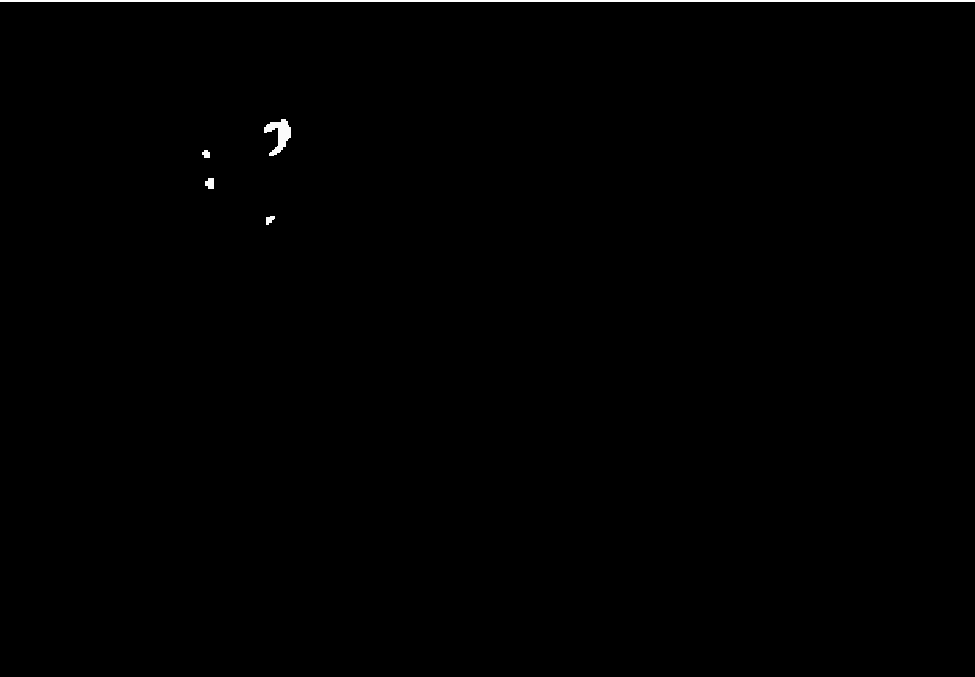
\includegraphics{tapas-vignette_files/figure-latex/unnamed-chunk-9-1.pdf}
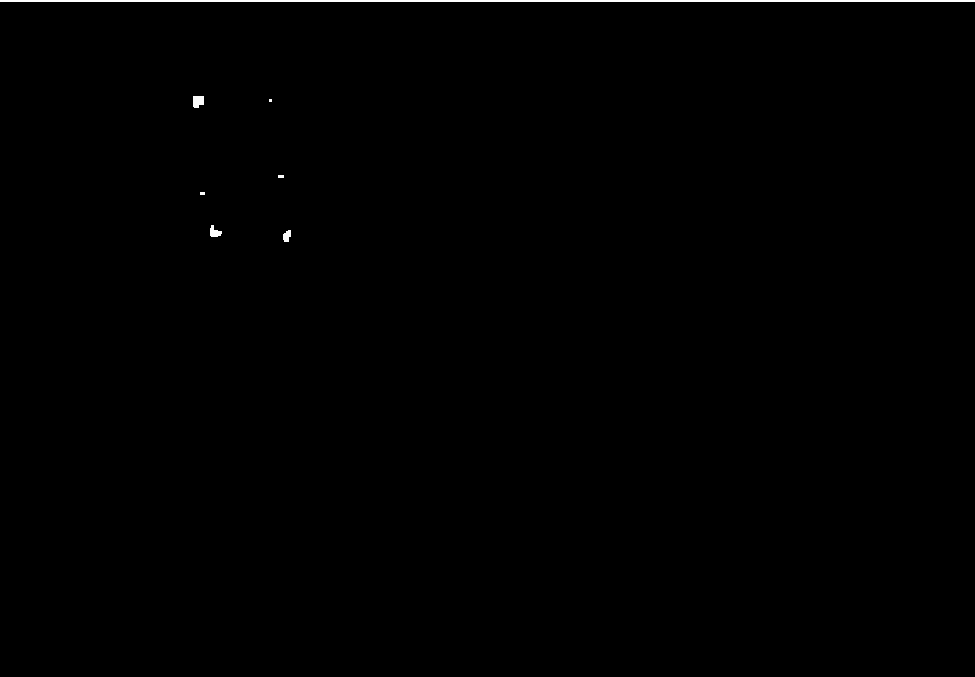
\includegraphics{tapas-vignette_files/figure-latex/unnamed-chunk-9-2.pdf}
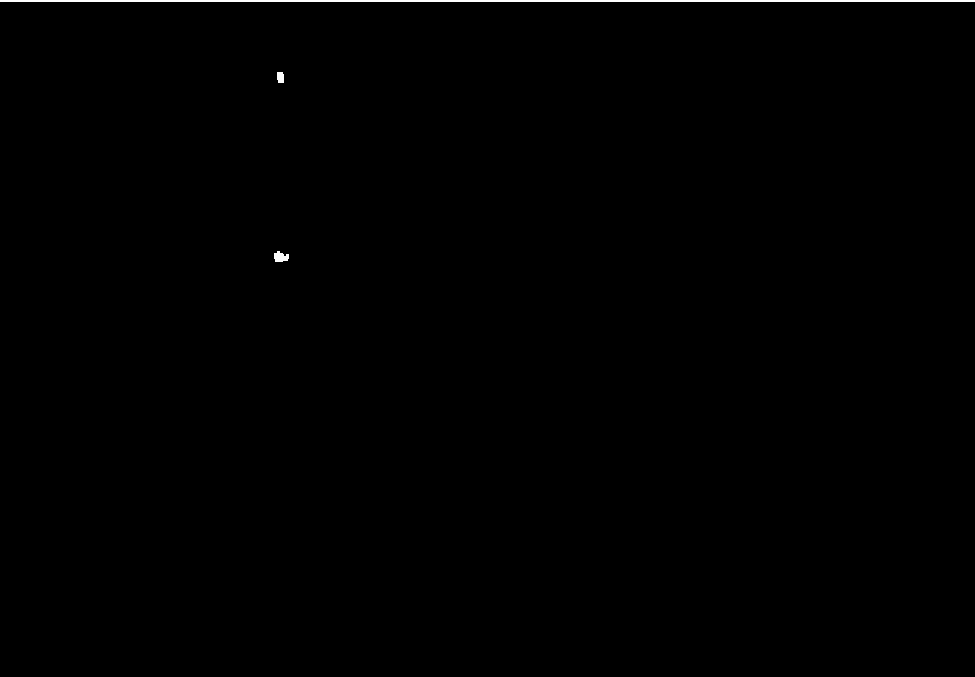
\includegraphics{tapas-vignette_files/figure-latex/unnamed-chunk-9-3.pdf}
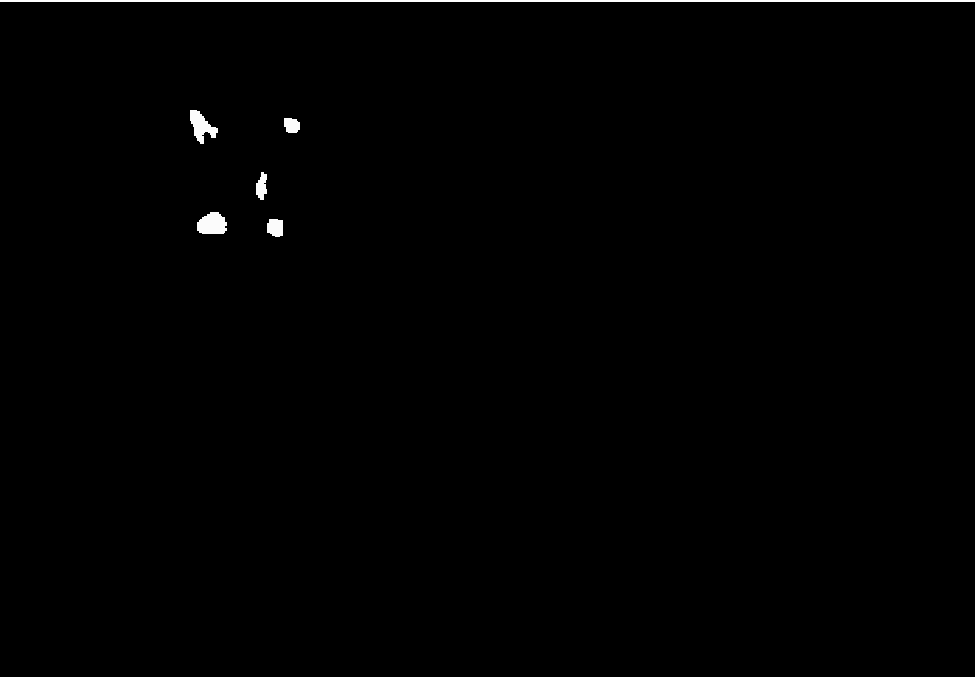
\includegraphics{tapas-vignette_files/figure-latex/unnamed-chunk-9-4.pdf}
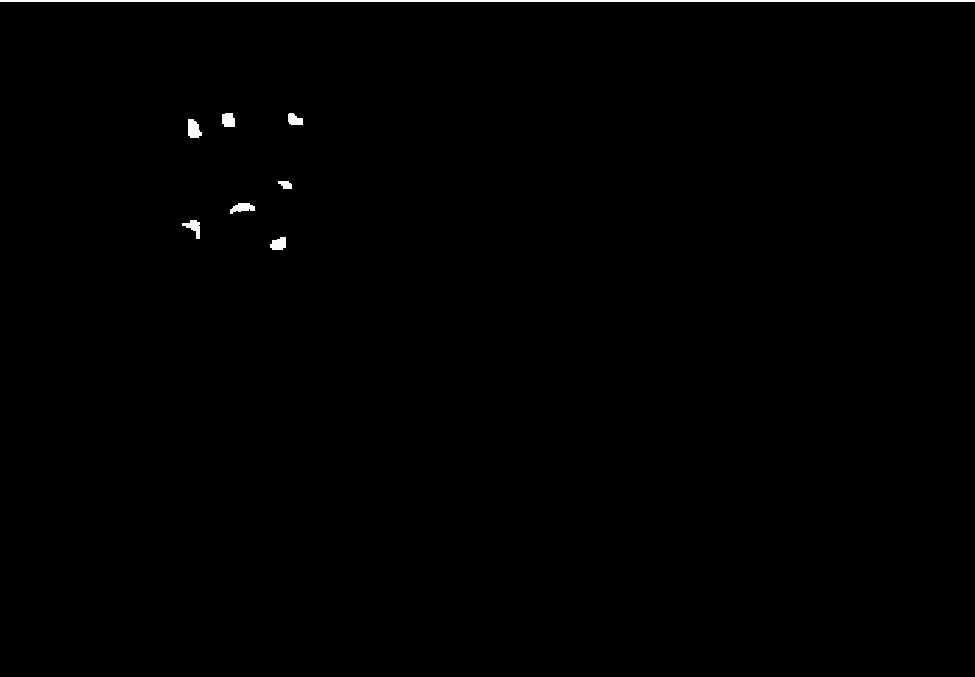
\includegraphics{tapas-vignette_files/figure-latex/unnamed-chunk-9-5.pdf}
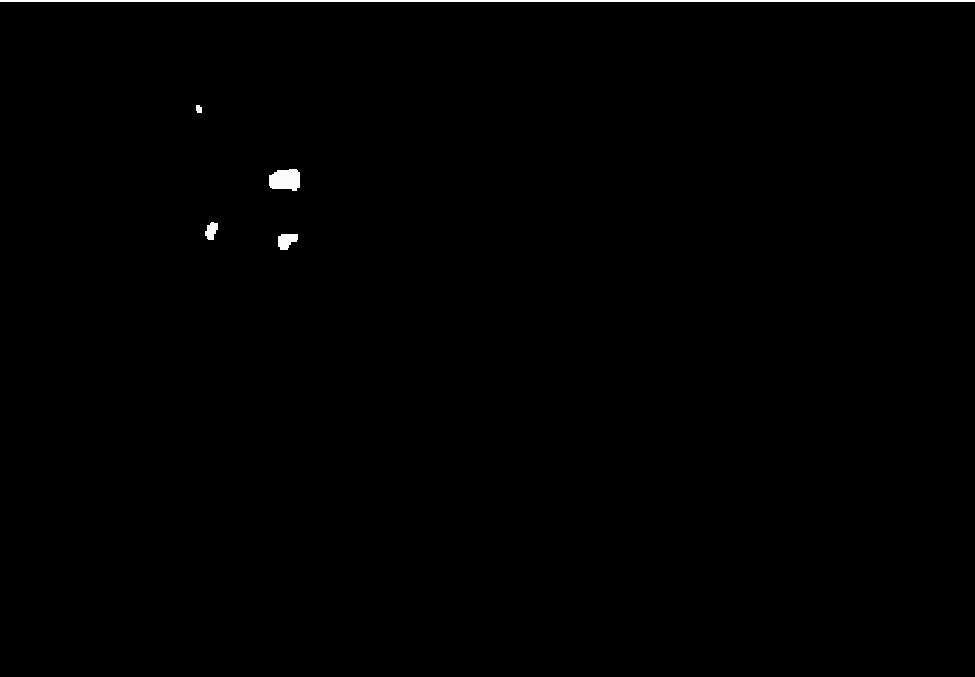
\includegraphics{tapas-vignette_files/figure-latex/unnamed-chunk-9-6.pdf}
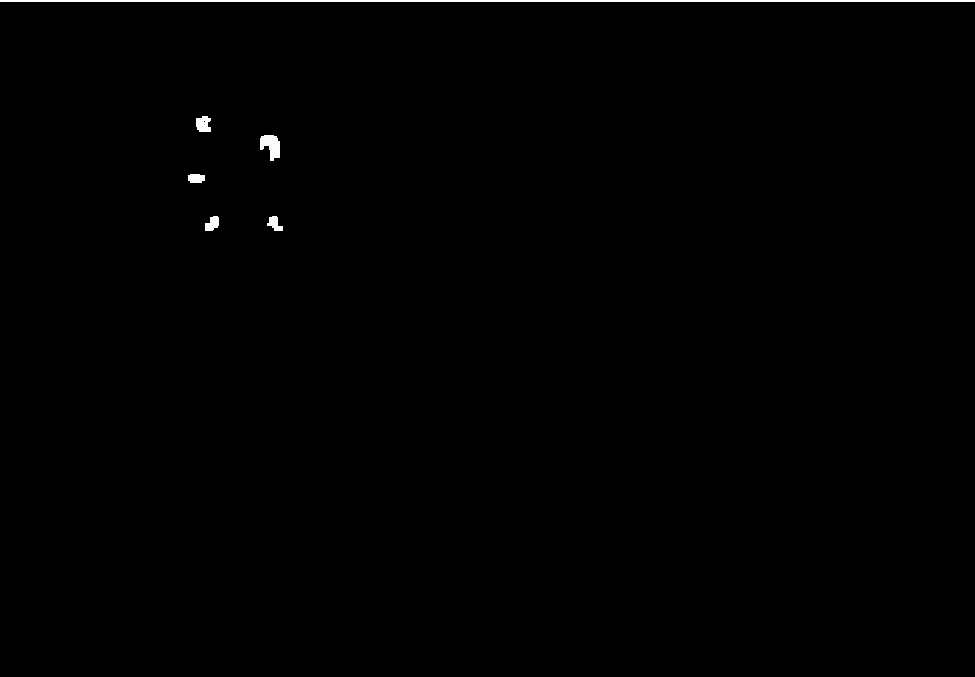
\includegraphics{tapas-vignette_files/figure-latex/unnamed-chunk-9-7.pdf}
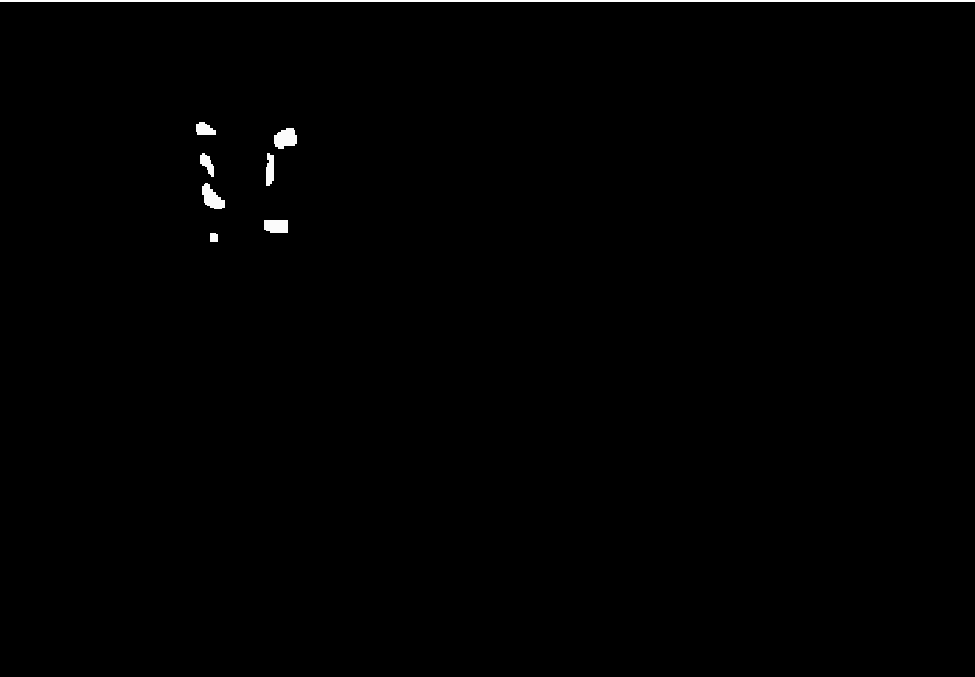
\includegraphics{tapas-vignette_files/figure-latex/unnamed-chunk-9-8.pdf}
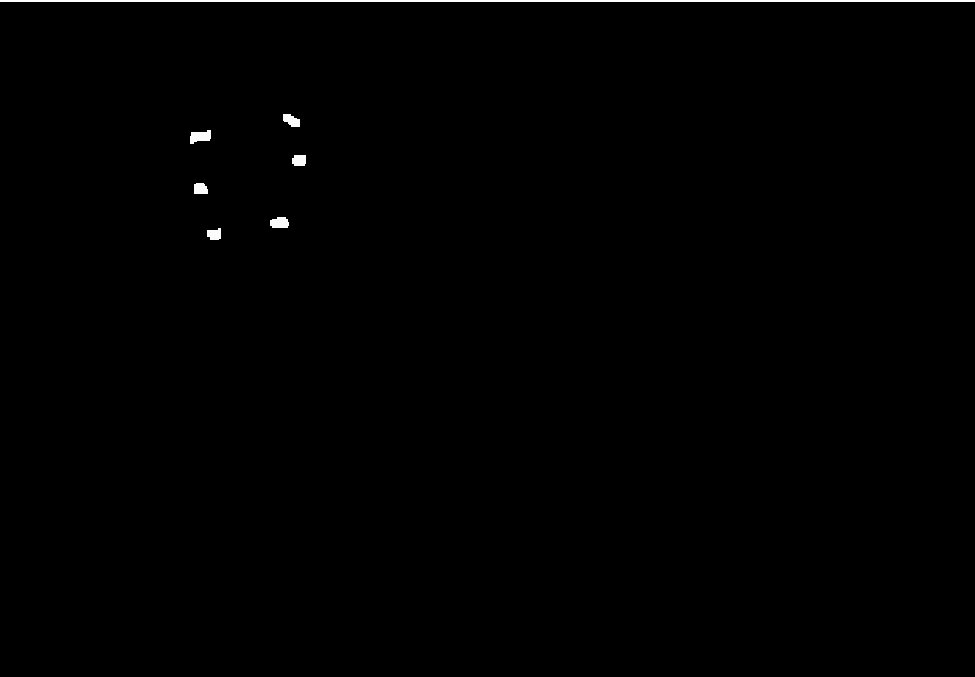
\includegraphics{tapas-vignette_files/figure-latex/unnamed-chunk-9-9.pdf}
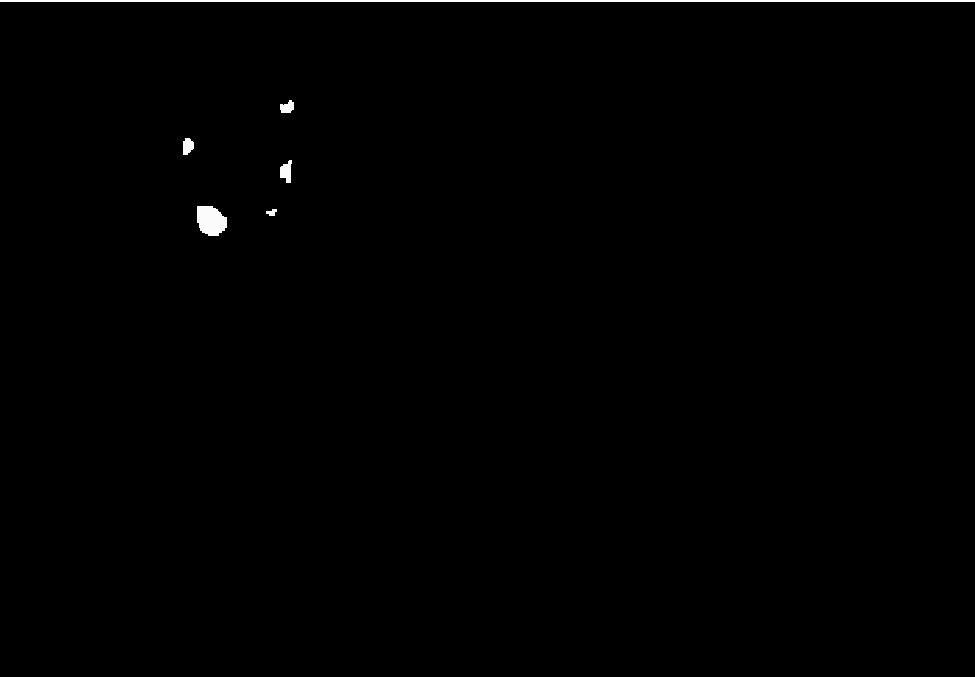
\includegraphics{tapas-vignette_files/figure-latex/unnamed-chunk-9-10.pdf}

\begin{verbatim}
#> integer(0)
\end{verbatim}

\hypertarget{training-probability-maps}{%
\subsection{Training Probability Maps}\label{training-probability-maps}}

The probability maps are all saved as \texttt{pmap\#}. We will use the
first 10 to train the TAPAS model.

\begin{Shaded}
\begin{Highlighting}[]
\CommentTok{# Make a list of the training probability maps}
\NormalTok{train_probability_maps =}\StringTok{ }\KeywordTok{list}\NormalTok{(}\DataTypeTok{pmap1 =}\NormalTok{ pmap1, }
                              \DataTypeTok{pmap2 =}\NormalTok{ pmap2, }
                              \DataTypeTok{pmap3 =}\NormalTok{ pmap3, }
                              \DataTypeTok{pmap4 =}\NormalTok{ pmap4, }
                              \DataTypeTok{pmap5 =}\NormalTok{ pmap5, }
                              \DataTypeTok{pmap6 =}\NormalTok{ pmap6, }
                              \DataTypeTok{pmap7 =}\NormalTok{ pmap7, }
                              \DataTypeTok{pmap8 =}\NormalTok{ pmap8, }
                              \DataTypeTok{pmap9 =}\NormalTok{ pmap9, }
                              \DataTypeTok{pmap10 =}\NormalTok{ pmap10)}

\CommentTok{# Convert the probability maps to nifti objects}
\NormalTok{train_probability_maps =}\StringTok{ }\KeywordTok{lapply}\NormalTok{(train_probability_maps, oro.nifti}\OperatorTok{::}\NormalTok{nifti)}
\end{Highlighting}
\end{Shaded}

The probability maps are visualized below:

\begin{Shaded}
\begin{Highlighting}[]
\CommentTok{# Show the probability maps using patchwork}
\NormalTok{oro.nifti}\OperatorTok{::}\KeywordTok{image}\NormalTok{(train_probability_maps}\OperatorTok{$}\NormalTok{pmap1, }\DataTypeTok{col =} \KeywordTok{heat.colors}\NormalTok{(}\DecValTok{100}\NormalTok{)) }\OperatorTok{+}\StringTok{ }
\StringTok{  }\NormalTok{oro.nifti}\OperatorTok{::}\KeywordTok{image}\NormalTok{(train_probability_maps}\OperatorTok{$}\NormalTok{pmap2, }\DataTypeTok{col =} \KeywordTok{heat.colors}\NormalTok{(}\DecValTok{100}\NormalTok{)) }\OperatorTok{+}\StringTok{ }
\StringTok{  }\NormalTok{oro.nifti}\OperatorTok{::}\KeywordTok{image}\NormalTok{(train_probability_maps}\OperatorTok{$}\NormalTok{pmap3, }\DataTypeTok{col =} \KeywordTok{heat.colors}\NormalTok{(}\DecValTok{100}\NormalTok{)) }\OperatorTok{+}\StringTok{ }
\StringTok{  }\NormalTok{oro.nifti}\OperatorTok{::}\KeywordTok{image}\NormalTok{(train_probability_maps}\OperatorTok{$}\NormalTok{pmap4, }\DataTypeTok{col =} \KeywordTok{heat.colors}\NormalTok{(}\DecValTok{100}\NormalTok{)) }\OperatorTok{+}
\StringTok{  }\NormalTok{oro.nifti}\OperatorTok{::}\KeywordTok{image}\NormalTok{(train_probability_maps}\OperatorTok{$}\NormalTok{pmap5, }\DataTypeTok{col =} \KeywordTok{heat.colors}\NormalTok{(}\DecValTok{100}\NormalTok{)) }\OperatorTok{+}\StringTok{ }
\StringTok{  }\NormalTok{oro.nifti}\OperatorTok{::}\KeywordTok{image}\NormalTok{(train_probability_maps}\OperatorTok{$}\NormalTok{pmap6, }\DataTypeTok{col =} \KeywordTok{heat.colors}\NormalTok{(}\DecValTok{100}\NormalTok{)) }\OperatorTok{+}
\StringTok{  }\NormalTok{oro.nifti}\OperatorTok{::}\KeywordTok{image}\NormalTok{(train_probability_maps}\OperatorTok{$}\NormalTok{pmap7, }\DataTypeTok{col =} \KeywordTok{heat.colors}\NormalTok{(}\DecValTok{100}\NormalTok{)) }\OperatorTok{+}\StringTok{ }
\StringTok{  }\NormalTok{oro.nifti}\OperatorTok{::}\KeywordTok{image}\NormalTok{(train_probability_maps}\OperatorTok{$}\NormalTok{pmap8, }\DataTypeTok{col =} \KeywordTok{heat.colors}\NormalTok{(}\DecValTok{100}\NormalTok{)) }\OperatorTok{+}
\StringTok{  }\NormalTok{oro.nifti}\OperatorTok{::}\KeywordTok{image}\NormalTok{(train_probability_maps}\OperatorTok{$}\NormalTok{pmap9, }\DataTypeTok{col =} \KeywordTok{heat.colors}\NormalTok{(}\DecValTok{100}\NormalTok{)) }\OperatorTok{+}
\StringTok{  }\NormalTok{oro.nifti}\OperatorTok{::}\KeywordTok{image}\NormalTok{(train_probability_maps}\OperatorTok{$}\NormalTok{pmap10, }\DataTypeTok{col =} \KeywordTok{heat.colors}\NormalTok{(}\DecValTok{100}\NormalTok{)) }
\end{Highlighting}
\end{Shaded}

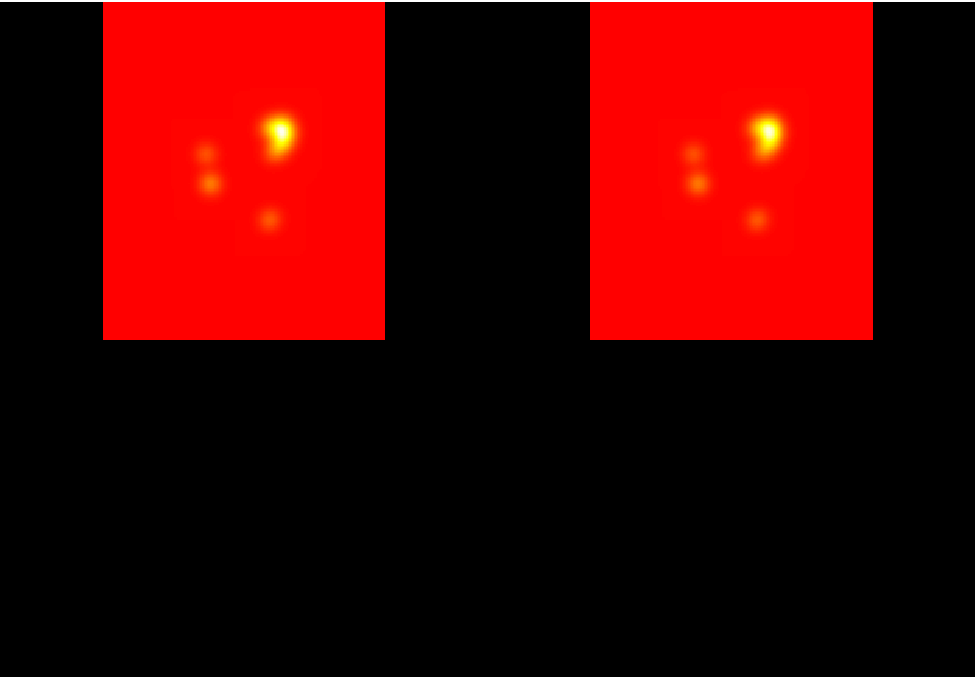
\includegraphics{tapas-vignette_files/figure-latex/unnamed-chunk-11-1.pdf}
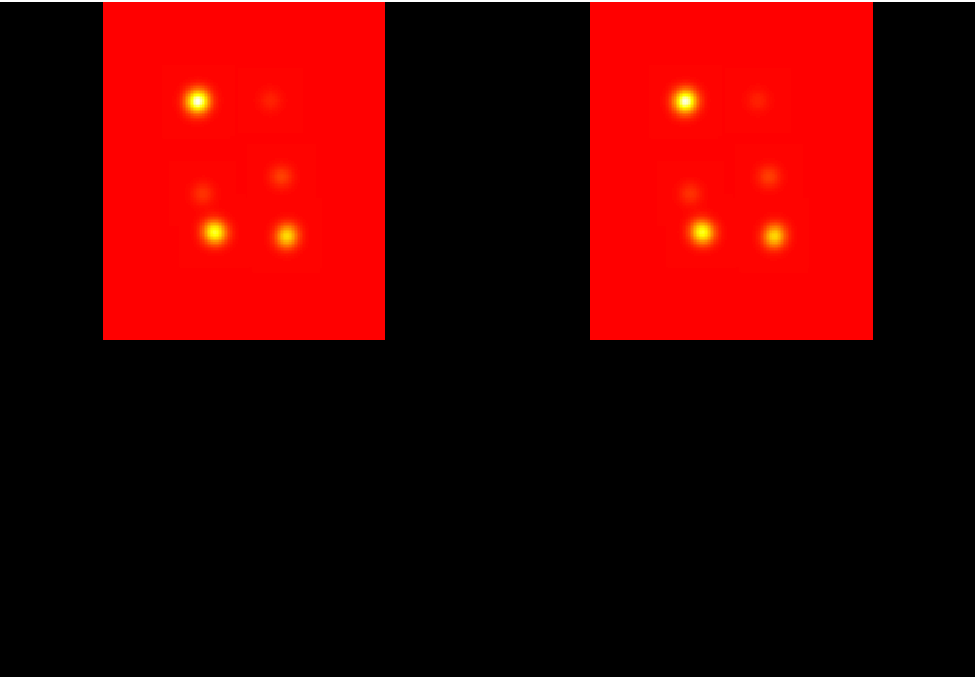
\includegraphics{tapas-vignette_files/figure-latex/unnamed-chunk-11-2.pdf}
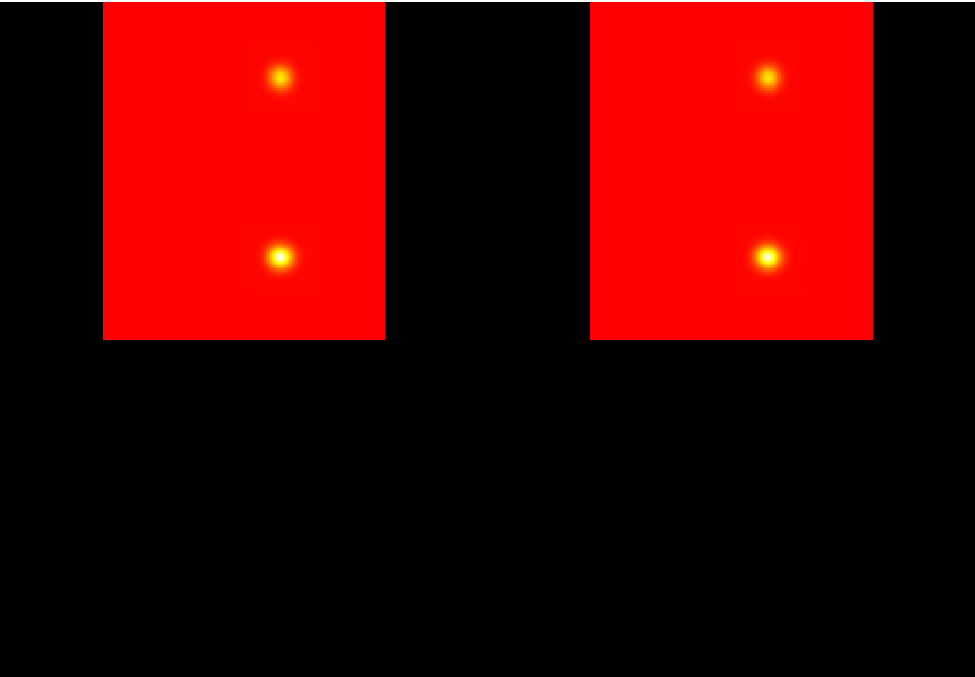
\includegraphics{tapas-vignette_files/figure-latex/unnamed-chunk-11-3.pdf}
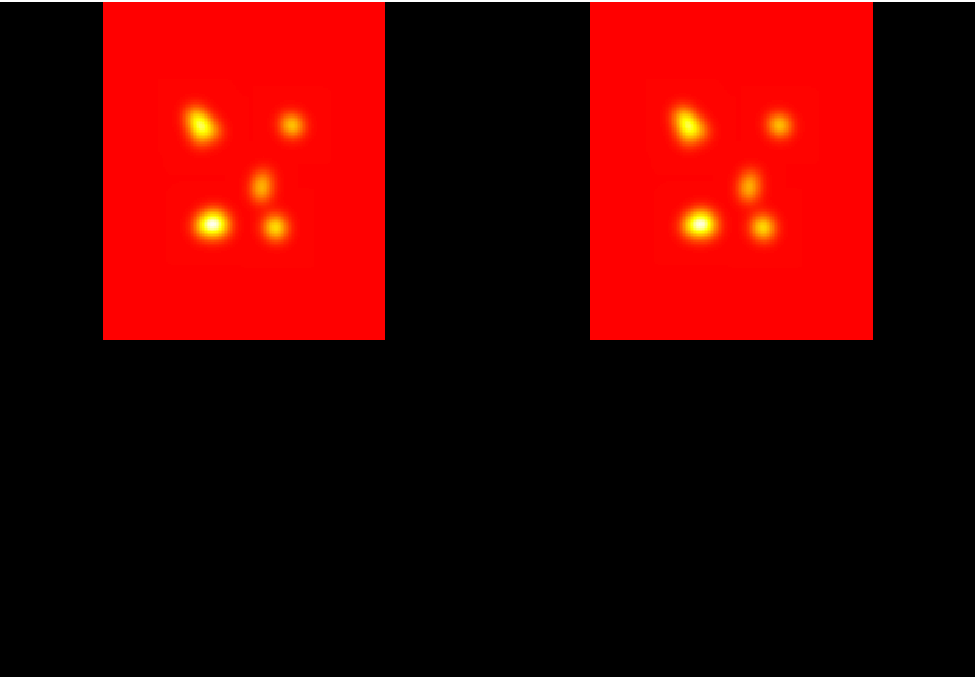
\includegraphics{tapas-vignette_files/figure-latex/unnamed-chunk-11-4.pdf}
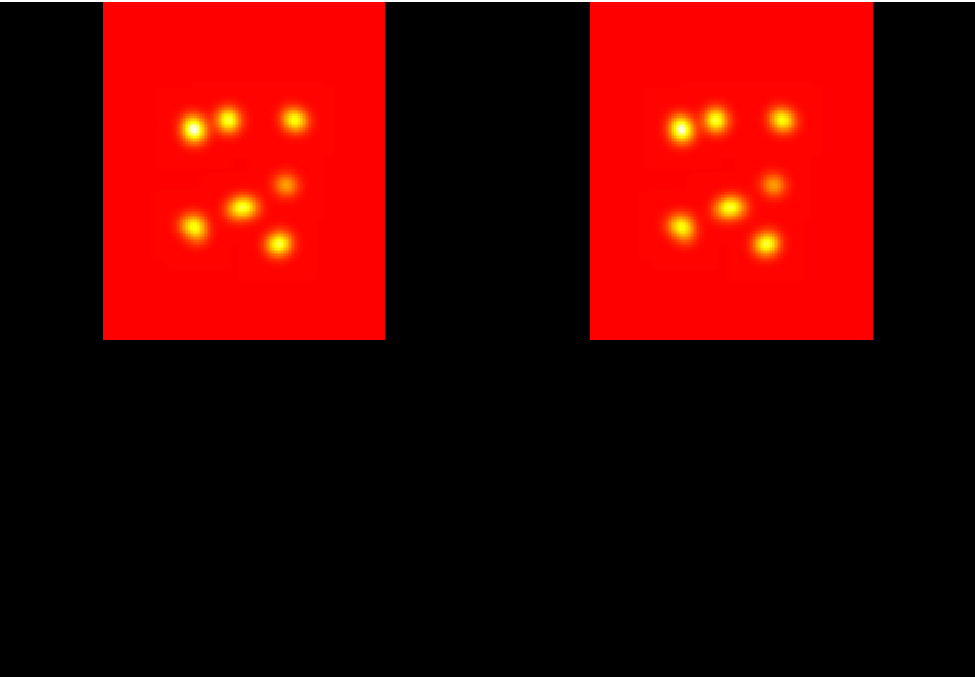
\includegraphics{tapas-vignette_files/figure-latex/unnamed-chunk-11-5.pdf}
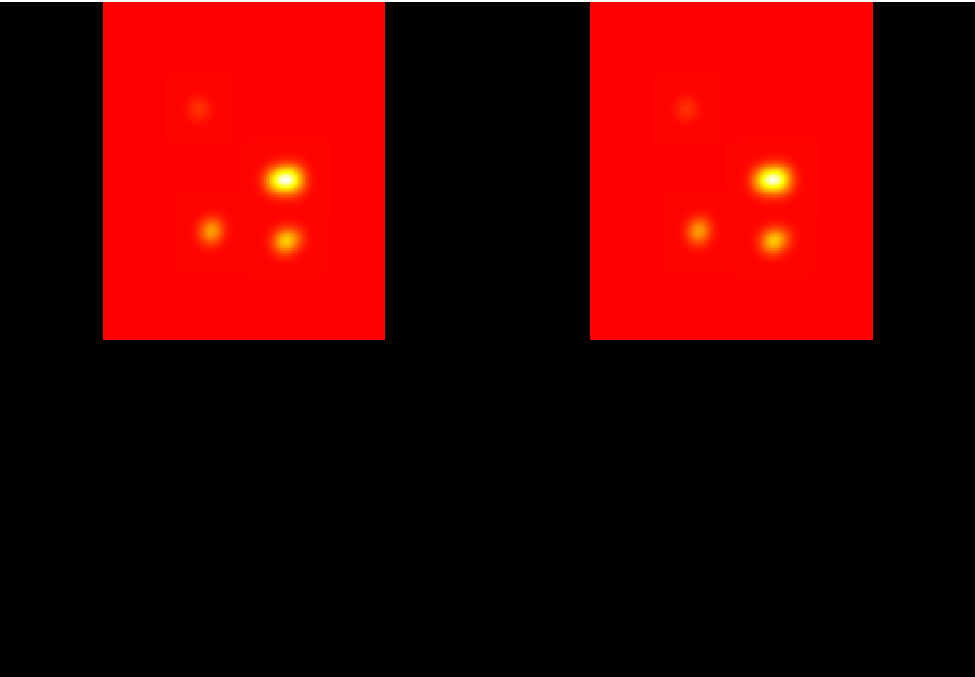
\includegraphics{tapas-vignette_files/figure-latex/unnamed-chunk-11-6.pdf}
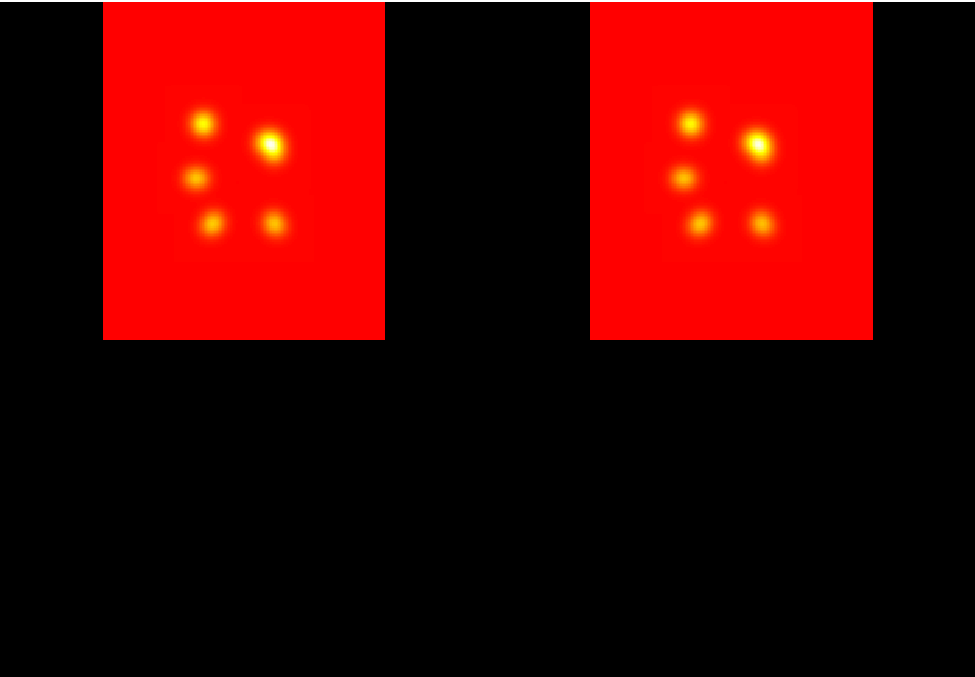
\includegraphics{tapas-vignette_files/figure-latex/unnamed-chunk-11-7.pdf}
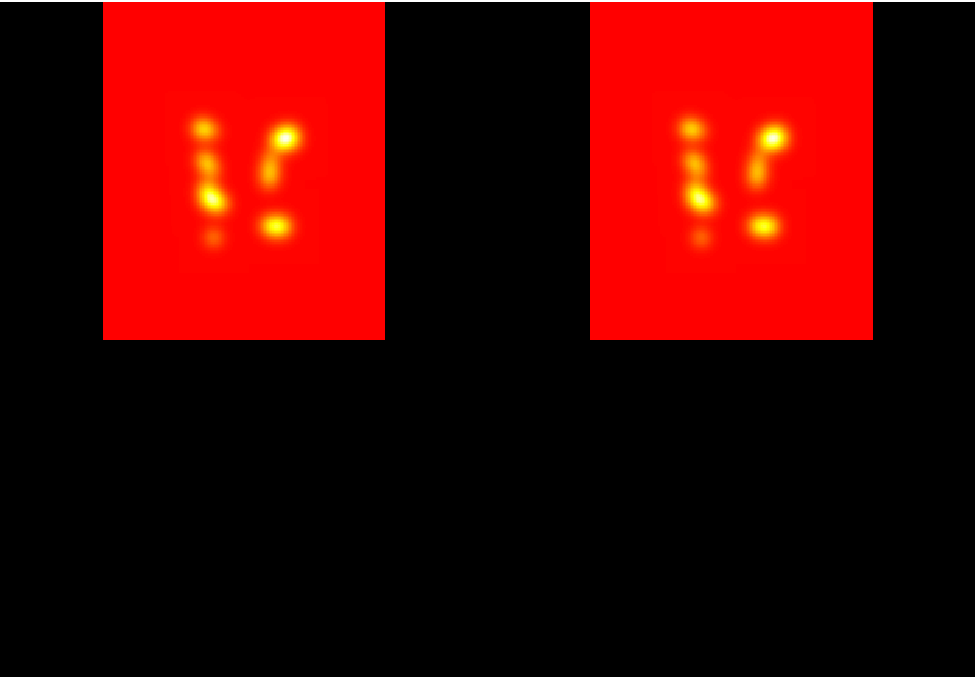
\includegraphics{tapas-vignette_files/figure-latex/unnamed-chunk-11-8.pdf}
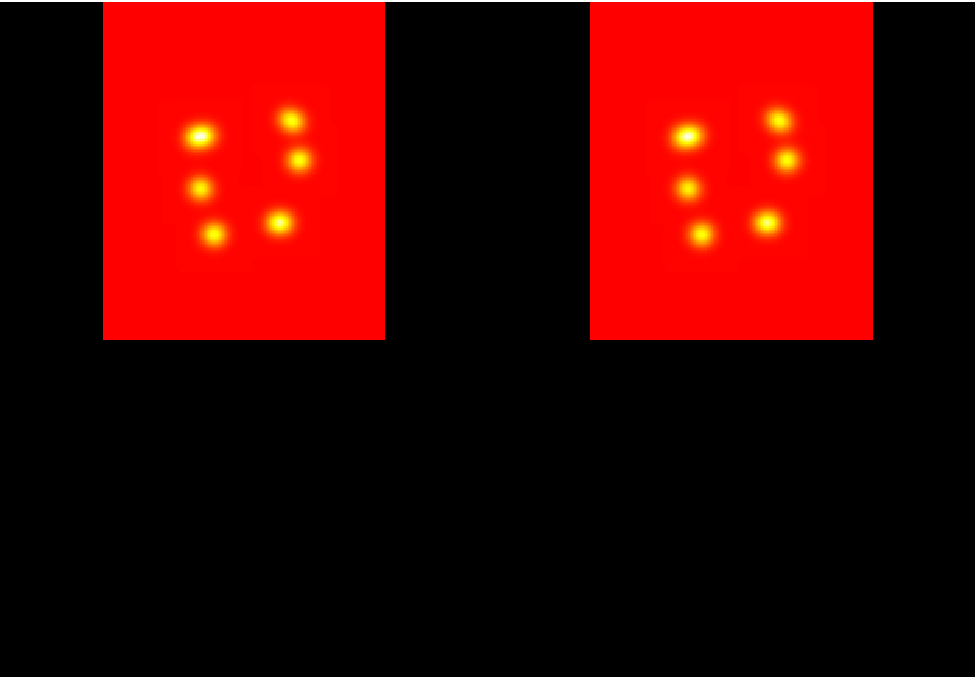
\includegraphics{tapas-vignette_files/figure-latex/unnamed-chunk-11-9.pdf}
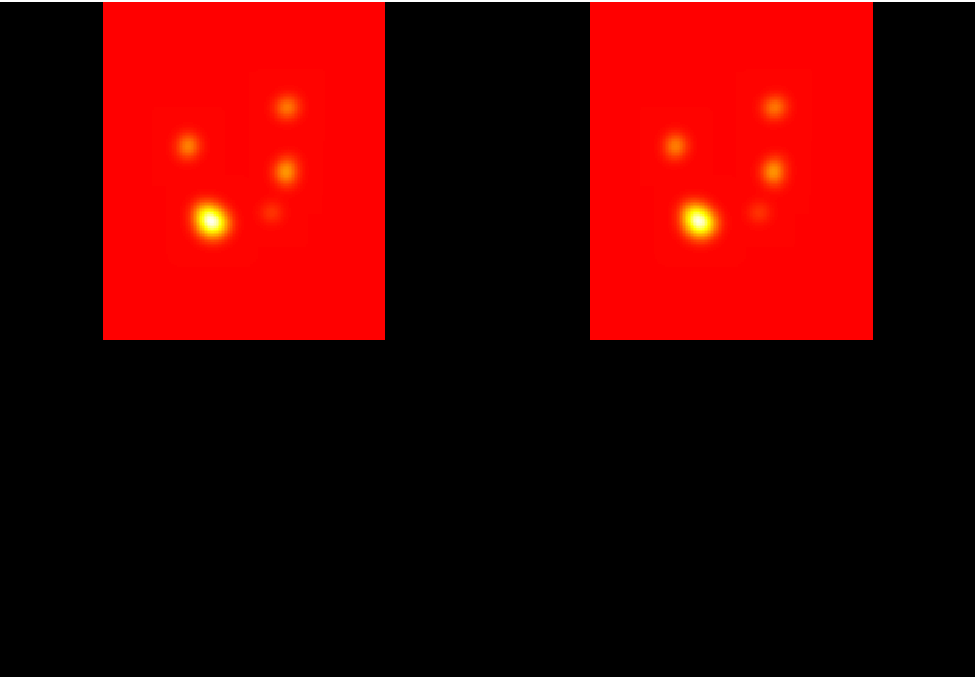
\includegraphics{tapas-vignette_files/figure-latex/unnamed-chunk-11-10.pdf}

\begin{verbatim}
#> integer(0)
\end{verbatim}

\hypertarget{training-brain-mask}{%
\subsection{Training Brain Mask}\label{training-brain-mask}}

There is only one brain mask included in the example data with this
package. This mask was created manually just to cover all the ``brain
matter'' in the gold standard masks and probability maps. Often each
subject will have a unique brain mask depending on the registration
technique. Below we create a list of brain masks so that the indices
match the indices of the gold standard list and probability map list.

\begin{Shaded}
\begin{Highlighting}[]
\CommentTok{# Make a list of the brain masks}
\NormalTok{train_brain_masks =}\StringTok{ }\KeywordTok{list}\NormalTok{(}\DataTypeTok{brain_mask1 =}\NormalTok{ brain_mask, }
                         \DataTypeTok{brain_mask2 =}\NormalTok{ brain_mask, }
                         \DataTypeTok{brain_mask3 =}\NormalTok{ brain_mask, }
                         \DataTypeTok{brain_mask4 =}\NormalTok{ brain_mask, }
                         \DataTypeTok{brain_mask5 =}\NormalTok{ brain_mask, }
                         \DataTypeTok{brain_mask6 =}\NormalTok{ brain_mask, }
                         \DataTypeTok{brain_mask7 =}\NormalTok{ brain_mask, }
                         \DataTypeTok{brain_mask8 =}\NormalTok{ brain_mask, }
                         \DataTypeTok{brain_mask9 =}\NormalTok{ brain_mask, }
                         \DataTypeTok{brain_mask10 =}\NormalTok{ brain_mask)}

\CommentTok{# Convert the brain masks to nifti objects}
\NormalTok{train_brain_masks =}\StringTok{ }\KeywordTok{lapply}\NormalTok{(train_brain_masks, oro.nifti}\OperatorTok{::}\NormalTok{nifti)}
\end{Highlighting}
\end{Shaded}

\hypertarget{training-subject-id}{%
\subsection{Training Subject ID}\label{training-subject-id}}

We will also need a vector of subject IDs to include. We simply create
an ID vector below:

\begin{Shaded}
\begin{Highlighting}[]
\NormalTok{train_ids =}\StringTok{ }\KeywordTok{paste0}\NormalTok{(}\StringTok{'subject_'}\NormalTok{, }\DecValTok{1}\OperatorTok{:}\KeywordTok{length}\NormalTok{(train_gold_standard_masks))}
\end{Highlighting}
\end{Shaded}

\hypertarget{generating-tapas-model-data}{%
\section{Generating TAPAS Model
Data}\label{generating-tapas-model-data}}

Before we can fit the TAPAS model, we have to generate the threshold
data required for model input. The model requires the Sørensen--Dice
coefficient value evaluated across all \texttt{thresholds} values for
each subject in the training set. We suggest evaluating thresholds from
0 to 1 by 1\% increments. This can be carried out using two functions:
\texttt{tapas\_data} and \texttt{tapas\_data\_par}. The
\texttt{tapas\_data} function will produce the model data for a single
subject whereas \texttt{tapas\_data\_par} is a wrapper around
\texttt{tapas\_data} and will run in parallel for multiple subjects.

Below we will calculate the TAPAS model input data using the example
data subject by subject using \texttt{tapas\_data}. We implement a
\texttt{for} loop for simplicity. The \texttt{pmap},
\texttt{gold\_standard}, and \texttt{mask} inputs must be either a local
object of class \texttt{nifti} or a vector of file paths to a
\texttt{nifti} object. The \texttt{subject\_id} is simply a vector of
subject IDs. These can be character or numeric. For this example we set
\texttt{k\ =\ 0} since the data is only a single slice of segmented
values and probability maps were randomly generated from a uniform. The
\texttt{thresholds} and \texttt{verbose} inputs are all set to the
default.

\begin{Shaded}
\begin{Highlighting}[]
\CommentTok{# Initialize an empty list to store results created on 1 core}
\NormalTok{train_data1 =}\StringTok{ }\KeywordTok{list}\NormalTok{()}

\CommentTok{# Run tapas_data function}
\ControlFlowTok{for}\NormalTok{(i }\ControlFlowTok{in} \DecValTok{1}\OperatorTok{:}\KeywordTok{length}\NormalTok{(train_probability_maps))\{}
\NormalTok{  train_data1[[i]] =}\StringTok{ }\KeywordTok{tapas_data}\NormalTok{(}\DataTypeTok{thresholds =} \KeywordTok{seq}\NormalTok{(}\DataTypeTok{from =} \DecValTok{0}\NormalTok{, }\DataTypeTok{to =} \DecValTok{1}\NormalTok{, }\DataTypeTok{by =} \FloatTok{0.01}\NormalTok{),}
                         \DataTypeTok{pmap =}\NormalTok{ train_probability_maps[[i]],}
                         \DataTypeTok{gold_standard =}\NormalTok{ train_gold_standard_masks[[i]],}
                         \DataTypeTok{mask =}\NormalTok{ train_brain_masks[[i]],}
                         \DataTypeTok{k =} \DecValTok{0}\NormalTok{,}
                         \DataTypeTok{subject_id =}\NormalTok{ train_ids[[i]],}
                         \DataTypeTok{verbose =} \OtherTok{TRUE}\NormalTok{)}
\NormalTok{\}}
\end{Highlighting}
\end{Shaded}

The \texttt{tapas\_data\_par} function simply is a parallel wrapper
around \texttt{tapas\_data}. Before we look at the return objects from
these functions let's replicate the results from \texttt{tapas\_data}
using \texttt{tapas\_data\_par} with 2 cores. The
\texttt{tapas\_data\_par} function is compatible with on both Unix and
Windows machines. Again, the code below is going to run on 2 cores so be
sure your machine has access to 2 cores or reduce back down to 1.

The inputs for \texttt{tapas\_data\_par} are similar to the
\texttt{tapas\_data} function but instead of single subject values we
use either a \texttt{list} of \texttt{nifti} objects or a
\texttt{vector} of file paths to \texttt{nifti} objects. By setting
\texttt{ret\ =\ TRUE} the subject TAPAS data generated by the wrapped
\texttt{tapas\_data} function will be returned locally in as a
\texttt{list}. This object may be extremely large depending on the
number of subjects used for training so be aware of memory constraints
if returning these objects locally. By default \texttt{outfile\ =\ NULL}
and the subject-level TAPAS data generated will not be saved out. If
users would like to save the subject-level data out then users must
specify a vector of file paths with \texttt{.rda} or \texttt{.RData}
file extensions included. Be sure that across \texttt{list} and
\texttt{vector} inputs the subject-level information is sorted and
consistent across each input.

\begin{Shaded}
\begin{Highlighting}[]
\CommentTok{# Store results created on 2 cores}
\CommentTok{# Run tapas_data_par function}
\NormalTok{train_data2 =}\StringTok{ }\KeywordTok{tapas_data_par}\NormalTok{(}\DataTypeTok{cores =} \DecValTok{2}\NormalTok{, }
                             \DataTypeTok{thresholds =} \KeywordTok{seq}\NormalTok{(}\DataTypeTok{from =} \DecValTok{0}\NormalTok{, }\DataTypeTok{to =} \DecValTok{1}\NormalTok{, }\DataTypeTok{by =} \FloatTok{0.01}\NormalTok{), }
                             \DataTypeTok{pmap =}\NormalTok{ train_probability_maps, }
                             \DataTypeTok{gold_standard =}\NormalTok{ train_gold_standard_masks, }
                             \DataTypeTok{mask =}\NormalTok{ train_brain_masks, }
                             \DataTypeTok{k =} \DecValTok{0}\NormalTok{, }
                             \DataTypeTok{subject_id =}\NormalTok{ train_ids,}
                             \DataTypeTok{ret =} \OtherTok{TRUE}\NormalTok{, }
                             \DataTypeTok{outfile =} \OtherTok{NULL}\NormalTok{, }
                             \DataTypeTok{verbose =} \OtherTok{TRUE}\NormalTok{)}
\end{Highlighting}
\end{Shaded}

The data produced using these functions is exactly the same. The only
difference is whether users would like to utilize parallel computing.

\begin{Shaded}
\begin{Highlighting}[]
\CommentTok{# Bind the single core data across list objects (subjects)}
\NormalTok{train_data1 =}\StringTok{ }\NormalTok{dplyr}\OperatorTok{::}\KeywordTok{bind_rows}\NormalTok{(train_data1)}
\CommentTok{# Bind the 2 core data across list objects (subjects)}
\NormalTok{train_data2 =}\StringTok{ }\NormalTok{dplyr}\OperatorTok{::}\KeywordTok{bind_rows}\NormalTok{(train_data2)}
\CommentTok{# Check that datasets are equal}
\KeywordTok{all.equal}\NormalTok{(train_data1, train_data2)}
\CommentTok{#> [1] TRUE}
\end{Highlighting}
\end{Shaded}

The data returned from either of these functions is needed to train the
TAPAS model. The \texttt{tapas\_data} function returns a single subject
level tibble while the \texttt{tapas\_data\_par} returns a list with
each subject-level tibble as an element in the list (only if
\texttt{ret\ =\ TRUE}). Each subject-level tibble contains the following
columns: \texttt{threshold}, \texttt{dsc}, \texttt{volume}, and
\texttt{subject\_id}. The first and last 5 rows of \texttt{train\_data1}
are shown below:

\begin{Shaded}
\begin{Highlighting}[]
\KeywordTok{head}\NormalTok{(train_data1)}
\CommentTok{#> # A tibble: 6 x 4}
\CommentTok{#>   threshold    dsc volume subject_id}
\CommentTok{#>       <dbl>  <dbl>  <dbl> <chr>     }
\CommentTok{#> 1      0    0.0325  16282 subject_1 }
\CommentTok{#> 2      0.01 0.124    4056 subject_1 }
\CommentTok{#> 3      0.02 0.165    2997 subject_1 }
\CommentTok{#> 4      0.03 0.210    2296 subject_1 }
\CommentTok{#> 5      0.04 0.258    1817 subject_1 }
\CommentTok{#> 6      0.05 0.314    1437 subject_1}
\KeywordTok{tail}\NormalTok{(train_data1)}
\CommentTok{#> # A tibble: 6 x 4}
\CommentTok{#>   threshold   dsc volume subject_id}
\CommentTok{#>       <dbl> <dbl>  <dbl> <chr>     }
\CommentTok{#> 1      0.95     0      0 subject_10}
\CommentTok{#> 2      0.96     0      0 subject_10}
\CommentTok{#> 3      0.97     0      0 subject_10}
\CommentTok{#> 4      0.98     0      0 subject_10}
\CommentTok{#> 5      0.99     0      0 subject_10}
\CommentTok{#> 6      1        0      0 subject_10}
\end{Highlighting}
\end{Shaded}

\hypertarget{fit-the-tapas-model}{%
\section{Fit the TAPAS Model}\label{fit-the-tapas-model}}

After the TAPAS data is generated using either \texttt{tapas\_data} or
\texttt{tapas\_data\_par} the TAPAS model can be fit using the
\texttt{tapas\_train} function. The subject training data must either be
a binded \texttt{tibble} or \texttt{data.frame} or a list with each
element the subject data. Previously, we binded the data together to
compare \texttt{train\_data1} and \texttt{train\_data2} so we will use
the \texttt{tibble} produced from above. We did this above when checking
that \texttt{train\_data1} and \texttt{train\_data2} are equal.

\begin{Shaded}
\begin{Highlighting}[]
\NormalTok{tapas_model =}\StringTok{ }\KeywordTok{tapas_train}\NormalTok{(}\DataTypeTok{data =}\NormalTok{ train_data1, }
                          \DataTypeTok{dsc_cutoff =} \FloatTok{0.03}\NormalTok{, }
                          \DataTypeTok{verbose =} \OtherTok{TRUE}\NormalTok{)}
\end{Highlighting}
\end{Shaded}

The return object from running \texttt{tapas\_train} includes a list
with the model in the named element \texttt{tapas\_model}, the group
threshold in the named element \texttt{group\_threshold}, and the
information about the clamping thresholds in the element
\texttt{clamp\_data}. Let's look at these objects:

\begin{Shaded}
\begin{Highlighting}[]
\CommentTok{# The TAPAS GAM model}
\KeywordTok{summary}\NormalTok{(tapas_model}\OperatorTok{$}\NormalTok{tapas_model)}
\CommentTok{#> }
\CommentTok{#> Family: gaussian }
\CommentTok{#> Link function: identity }
\CommentTok{#> }
\CommentTok{#> Formula:}
\CommentTok{#> gtools::logit(threshold) ~ s(volume)}
\CommentTok{#> }
\CommentTok{#> Parametric coefficients:}
\CommentTok{#>             Estimate Std. Error t value Pr(>|t|)    }
\CommentTok{#> (Intercept) -2.07312    0.08166  -25.39 7.71e-09 ***}
\CommentTok{#> ---}
\CommentTok{#> Signif. codes:  0 '***' 0.001 '**' 0.01 '*' 0.05 '.' 0.1 ' ' 1}
\CommentTok{#> }
\CommentTok{#> Approximate significance of smooth terms:}
\CommentTok{#>             edf Ref.df     F p-value  }
\CommentTok{#> s(volume) 1.122  1.233 7.126  0.0286 *}
\CommentTok{#> ---}
\CommentTok{#> Signif. codes:  0 '***' 0.001 '**' 0.01 '*' 0.05 '.' 0.1 ' ' 1}
\CommentTok{#> }
\CommentTok{#> R-sq.(adj) =  0.448   Deviance explained = 51.7%}
\CommentTok{#> GCV = 0.084654  Scale est. = 0.066687  n = 10}
\CommentTok{# The threshold that optimizes group-level DSC}
\NormalTok{tapas_model}\OperatorTok{$}\NormalTok{group_threshold}
\CommentTok{#> [1] 0.09}
\CommentTok{# The lower and upper bound clamps to avoid extrapolation}
\NormalTok{tapas_model}\OperatorTok{$}\NormalTok{clamp_data}
\CommentTok{#> # A tibble: 2 x 3}
\CommentTok{#>   bound volume pred_threshold}
\CommentTok{#>   <chr>  <dbl>          <dbl>}
\CommentTok{#> 1 lower   154.         0.0868}
\CommentTok{#> 2 upper  2280.         0.153}
\end{Highlighting}
\end{Shaded}

We can use this model to predict a subject-specific thresholds, create a
segmentation mask using this threshold, and create a segmentation mask
using the group-threshold for a subjects not included in model training.

\hypertarget{load-testing-data}{%
\section{Load Testing Data}\label{load-testing-data}}

To use the data throughout the testing of the model we will initialize
the remaining 5 gold standard masks, 5 probability maps, and 5 brain
masks not used in the training procedure into a list.

\hypertarget{testing-gold-standard-masks}{%
\subsection{Testing Gold Standard
Masks}\label{testing-gold-standard-masks}}

The gold standard masks are all saved as \texttt{gs\#}. We will use the
last 5 to train the TAPAS model.

\begin{Shaded}
\begin{Highlighting}[]
\CommentTok{# Testing gold standard masks}
\NormalTok{test_gold_standard_masks =}\StringTok{ }\KeywordTok{list}\NormalTok{(}\DataTypeTok{gs11 =}\NormalTok{ gs11,}
                                \DataTypeTok{gs12 =}\NormalTok{ gs12,}
                                \DataTypeTok{gs13 =}\NormalTok{ gs13,}
                                \DataTypeTok{gs14 =}\NormalTok{ gs14,}
                                \DataTypeTok{gs15 =}\NormalTok{ gs15)}

\CommentTok{# Make array objects niftis}
\NormalTok{test_gold_standard_masks =}\StringTok{ }\KeywordTok{lapply}\NormalTok{(test_gold_standard_masks, oro.nifti}\OperatorTok{::}\NormalTok{nifti)}

\CommentTok{# Visualize the testing subjects gold standard masks}
\NormalTok{oro.nifti}\OperatorTok{::}\KeywordTok{image}\NormalTok{(test_gold_standard_masks}\OperatorTok{$}\NormalTok{gs11) }\OperatorTok{+}\StringTok{ }\NormalTok{oro.nifti}\OperatorTok{::}\KeywordTok{image}\NormalTok{(test_gold_standard_masks}\OperatorTok{$}\NormalTok{gs12) }\OperatorTok{+}
\NormalTok{oro.nifti}\OperatorTok{::}\KeywordTok{image}\NormalTok{(test_gold_standard_masks}\OperatorTok{$}\NormalTok{gs13) }\OperatorTok{+}\StringTok{ }\NormalTok{oro.nifti}\OperatorTok{::}\KeywordTok{image}\NormalTok{(test_gold_standard_masks}\OperatorTok{$}\NormalTok{gs14) }\OperatorTok{+}
\NormalTok{oro.nifti}\OperatorTok{::}\KeywordTok{image}\NormalTok{(test_gold_standard_masks}\OperatorTok{$}\NormalTok{gs15)}
\end{Highlighting}
\end{Shaded}

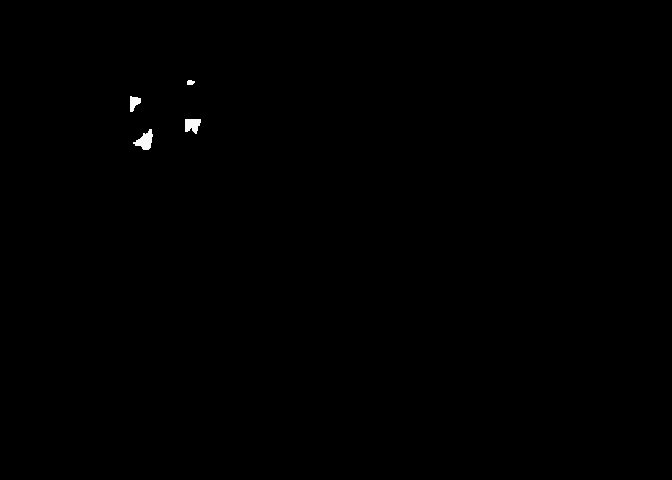
\includegraphics{tapas-vignette_files/figure-latex/unnamed-chunk-20-1.pdf}
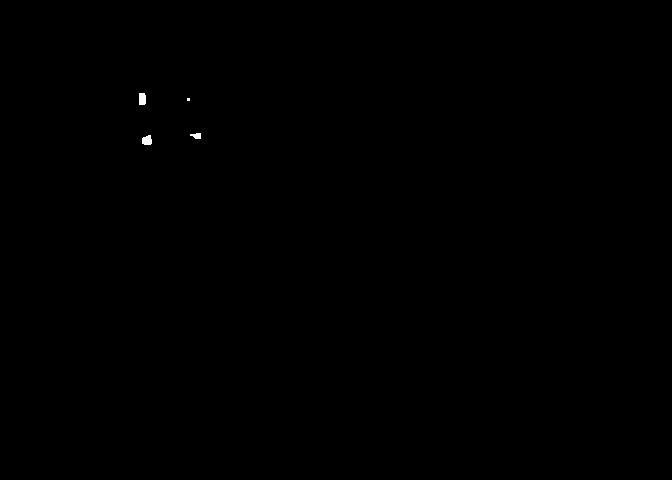
\includegraphics{tapas-vignette_files/figure-latex/unnamed-chunk-20-2.pdf}
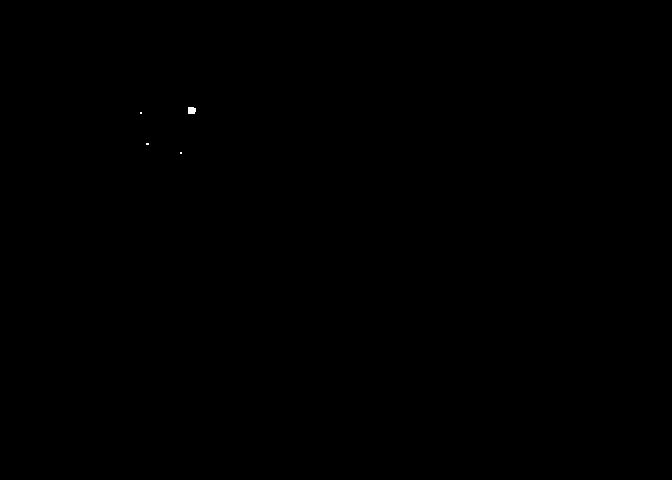
\includegraphics{tapas-vignette_files/figure-latex/unnamed-chunk-20-3.pdf}
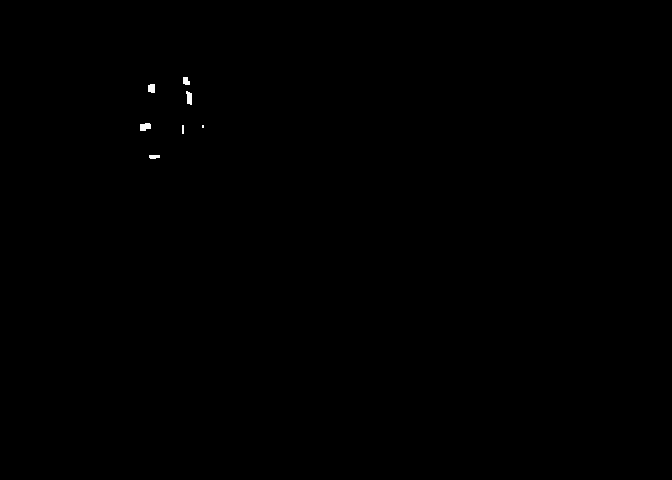
\includegraphics{tapas-vignette_files/figure-latex/unnamed-chunk-20-4.pdf}
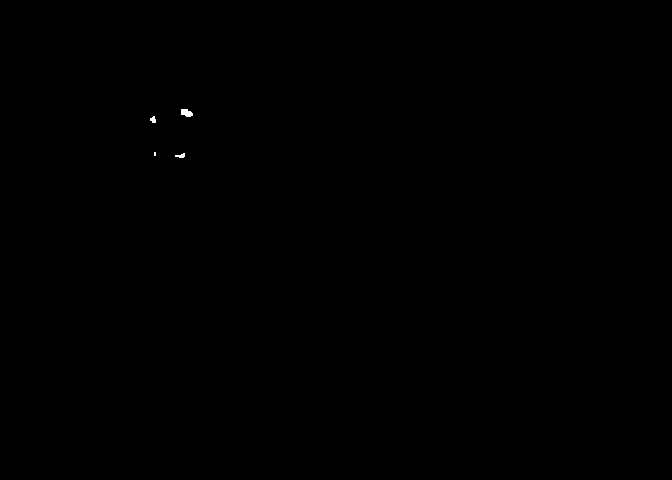
\includegraphics{tapas-vignette_files/figure-latex/unnamed-chunk-20-5.pdf}

\begin{verbatim}
#> integer(0)
\end{verbatim}

The gold standard segmentations are visualized below:

\hypertarget{testing-probability-maps}{%
\subsection{Testing Probability Maps}\label{testing-probability-maps}}

The probability maps are all saved as \texttt{pmap\#}. We will use the
last 5 to train the TAPAS model.

\begin{Shaded}
\begin{Highlighting}[]
\CommentTok{# Obtain the test subject probability maps}
\NormalTok{test_probability_maps =}\StringTok{ }\KeywordTok{list}\NormalTok{(}\DataTypeTok{pmap11 =}\NormalTok{ pmap11, }
                             \DataTypeTok{pmap12 =}\NormalTok{ pmap12,}
                             \DataTypeTok{pmap13 =}\NormalTok{ pmap13,}
                             \DataTypeTok{pmap14 =}\NormalTok{ pmap14,}
                             \DataTypeTok{pmap15 =}\NormalTok{ pmap15)}

\CommentTok{# Make array objects niftis}
\NormalTok{test_probability_maps =}\StringTok{ }\KeywordTok{lapply}\NormalTok{(test_probability_maps, oro.nifti}\OperatorTok{::}\NormalTok{nifti)}

\CommentTok{# Visualize the 5 testing probability maps}
\NormalTok{oro.nifti}\OperatorTok{::}\KeywordTok{image}\NormalTok{(test_probability_maps}\OperatorTok{$}\NormalTok{pmap11, }\DataTypeTok{col =} \KeywordTok{heat.colors}\NormalTok{(}\DecValTok{100}\NormalTok{)) }\OperatorTok{+}
\NormalTok{oro.nifti}\OperatorTok{::}\KeywordTok{image}\NormalTok{(test_probability_maps}\OperatorTok{$}\NormalTok{pmap12, }\DataTypeTok{col =} \KeywordTok{heat.colors}\NormalTok{(}\DecValTok{100}\NormalTok{)) }\OperatorTok{+}
\NormalTok{oro.nifti}\OperatorTok{::}\KeywordTok{image}\NormalTok{(test_probability_maps}\OperatorTok{$}\NormalTok{pmap13, }\DataTypeTok{col =} \KeywordTok{heat.colors}\NormalTok{(}\DecValTok{100}\NormalTok{)) }\OperatorTok{+}
\NormalTok{oro.nifti}\OperatorTok{::}\KeywordTok{image}\NormalTok{(test_probability_maps}\OperatorTok{$}\NormalTok{pmap14, }\DataTypeTok{col =} \KeywordTok{heat.colors}\NormalTok{(}\DecValTok{100}\NormalTok{)) }\OperatorTok{+}
\NormalTok{oro.nifti}\OperatorTok{::}\KeywordTok{image}\NormalTok{(test_probability_maps}\OperatorTok{$}\NormalTok{pmap15, }\DataTypeTok{col =} \KeywordTok{heat.colors}\NormalTok{(}\DecValTok{100}\NormalTok{))}
\end{Highlighting}
\end{Shaded}

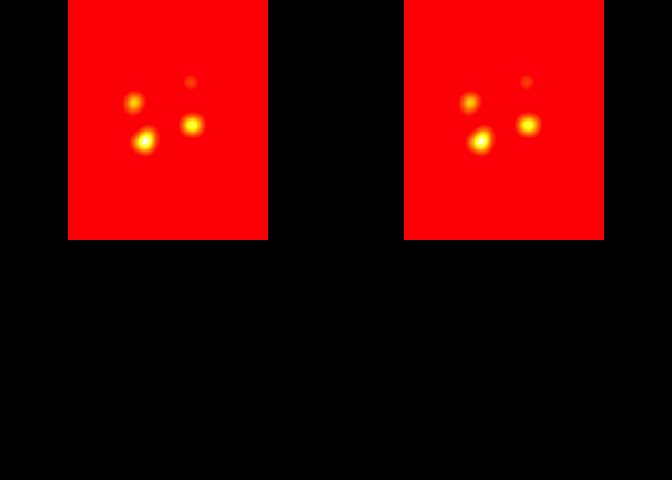
\includegraphics{tapas-vignette_files/figure-latex/unnamed-chunk-21-1.pdf}
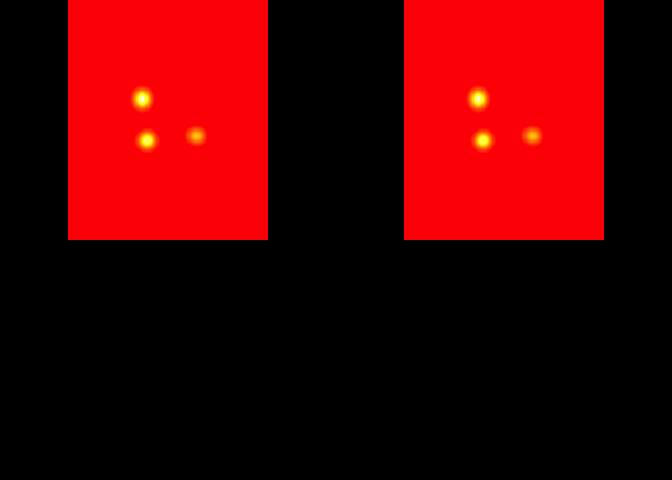
\includegraphics{tapas-vignette_files/figure-latex/unnamed-chunk-21-2.pdf}
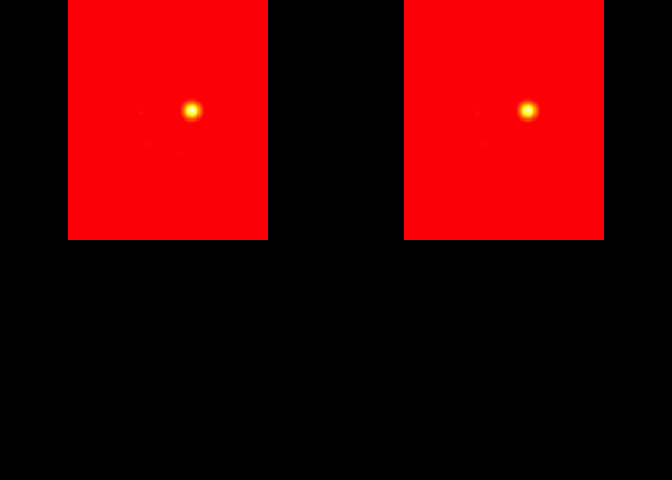
\includegraphics{tapas-vignette_files/figure-latex/unnamed-chunk-21-3.pdf}
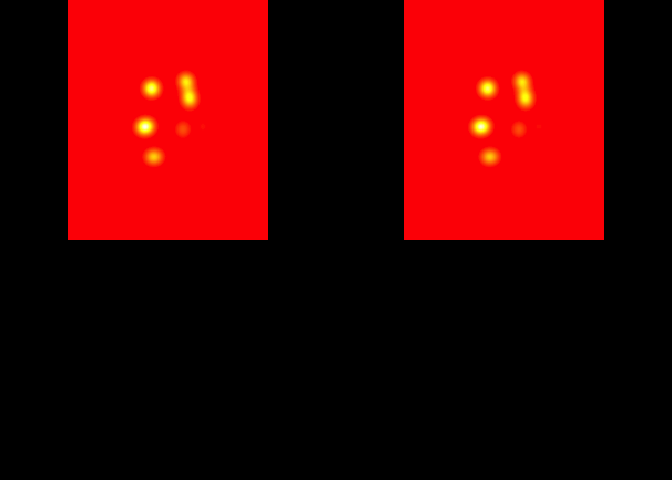
\includegraphics{tapas-vignette_files/figure-latex/unnamed-chunk-21-4.pdf}
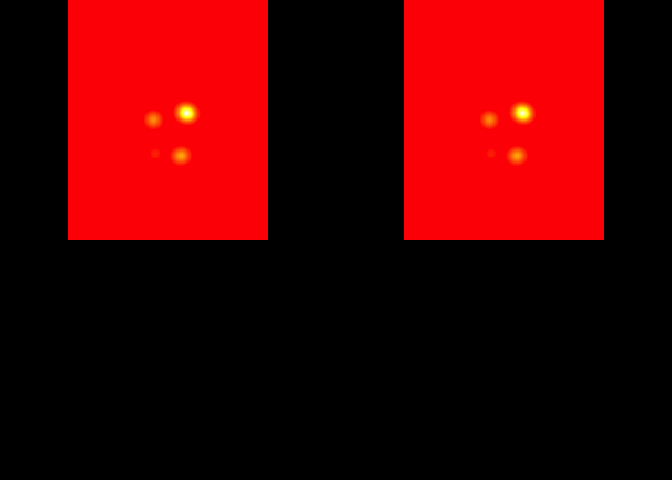
\includegraphics{tapas-vignette_files/figure-latex/unnamed-chunk-21-5.pdf}

\begin{verbatim}
#> integer(0)
\end{verbatim}

The probability maps are visualized below:

\hypertarget{testing-brain-masks}{%
\subsection{Testing Brain Masks}\label{testing-brain-masks}}

There is only one brain mask included in the example data with this
package. This mask was created manually just to cover all the ``brain
matter'' in the gold standard masks and probability maps. Often each
subject will have a unique brain mask depending on the registration
technique. Below we create a list of brain masks so that the indices
match the indices of the gold standard list and probability map list.

\begin{Shaded}
\begin{Highlighting}[]
\CommentTok{# Create a list of testing brain masks}
\NormalTok{test_brain_masks =}\StringTok{ }\KeywordTok{list}\NormalTok{(}\DataTypeTok{brain_mask11 =}\NormalTok{ brain_mask, }
                        \DataTypeTok{brain_mask12 =}\NormalTok{ brain_mask,}
                        \DataTypeTok{brain_mask13 =}\NormalTok{ brain_mask,}
                        \DataTypeTok{brain_mask14 =}\NormalTok{ brain_mask,}
                        \DataTypeTok{brain_mask15 =}\NormalTok{ brain_mask)}

\CommentTok{# Make array objects niftis}
\NormalTok{test_brain_masks =}\StringTok{ }\KeywordTok{lapply}\NormalTok{(test_brain_masks, oro.nifti}\OperatorTok{::}\NormalTok{nifti)}
\end{Highlighting}
\end{Shaded}

\hypertarget{testing-subject-id}{%
\subsection{Testing Subject ID}\label{testing-subject-id}}

We will also need a vector of subject IDs to include. We simply create
an ID vector below:

\begin{Shaded}
\begin{Highlighting}[]
\NormalTok{test_ids =}\StringTok{ }\KeywordTok{paste0}\NormalTok{(}\StringTok{'subject_'}\NormalTok{, (}\DecValTok{10} \OperatorTok{+}\StringTok{ }\DecValTok{1}\OperatorTok{:}\KeywordTok{length}\NormalTok{(test_gold_standard_masks)))}
\end{Highlighting}
\end{Shaded}

\hypertarget{predicting-thresholds-and-segmentation-masks}{%
\section{Predicting Thresholds and Segmentation
Masks}\label{predicting-thresholds-and-segmentation-masks}}

Below we will predict using the TAPAS model subject by subject using
\texttt{tapas\_predict}. We implement a \texttt{for} loop for
simplicity. The \texttt{pmap} and \texttt{mask} inputs must be either a
local object of class \texttt{nifti} or a vector of file paths to a
\texttt{nifti} object. The \texttt{subject\_id} is simply a vector of
subject IDs. These can be character or numeric. For this example we set
\texttt{k\ =\ 0} since the data is only a single slice of segmented
values and probability maps were randomly generated from a uniform. We
use the default \texttt{clamp\ =\ TRUE} which will use the threshold
associated with the 10th or 90th percentile volume from the training
data rather than the subject-specific fitted value. This is to avoid
extrapolation in the tails of the TAPAS model. The \texttt{verbose}
input is set to \texttt{TRUE}.

\begin{Shaded}
\begin{Highlighting}[]
\CommentTok{# Initialize an empty list to store results created on 1 core}
\NormalTok{test_data1 =}\StringTok{ }\KeywordTok{list}\NormalTok{()}

\CommentTok{# Run tapas_predict function}
\ControlFlowTok{for}\NormalTok{(i }\ControlFlowTok{in} \DecValTok{1}\OperatorTok{:}\KeywordTok{length}\NormalTok{(test_probability_maps))\{}
\NormalTok{  test_data1[[i]] =}\StringTok{ }\KeywordTok{tapas_predict}\NormalTok{(}\DataTypeTok{pmap =}\NormalTok{ test_probability_maps[[i]],}
                                  \DataTypeTok{model =}\NormalTok{ tapas_model,}
                                  \DataTypeTok{clamp =} \OtherTok{TRUE}\NormalTok{,}
                                  \DataTypeTok{k =} \DecValTok{0}\NormalTok{,}
                                  \DataTypeTok{verbose =} \OtherTok{TRUE}\NormalTok{)}
\NormalTok{\}}
\end{Highlighting}
\end{Shaded}

The \texttt{tapas\_predict\_par} function simply is a parallel wrapper
around \texttt{tapas\_predict}. Before we look at the return objects
from these functions let's replicate the results from
\texttt{tapas\_predict} using \texttt{tapas\_predict\_par} with 2 cores.
The \texttt{tapas\_predict\_par} function is compatible with on both
Unix and Windows machines. Again, the code below is going to run on 2
cores so be sure your machine has access to 2 cores or reduce back down
to 1.

The inputs for \texttt{tapas\_predict\_par} are similar to the
\texttt{tapas\_predict} function but instead of single subject values
include either a \texttt{list} of \texttt{nifti} objects or a
\texttt{vector} of file paths to \texttt{nifti} objects. By setting
\texttt{ret\ =\ TRUE} the TAPAS predicted subject data generated by the
wrapped \texttt{tapas\_predict} function will be returned locally as a
\texttt{list}. This object may be extremely large depending on the
number of subjects used for training so be aware of memory constraints
if returning these objects locally. By default \texttt{outfile\ =\ NULL}
and the predicted subject-level data generated will not be saved out. If
users would like to save the predicted subject-level data out then users
must specify a vector of file names with \texttt{.rda} or
\texttt{.RData} file extensions included. Be sure that across
\texttt{list} and \texttt{vector} inputs the subject-level information
is sorted and consistent across each input.

\begin{Shaded}
\begin{Highlighting}[]
\CommentTok{# Store results created on 2 cores}
\CommentTok{# Run tapas_predict_par function}
\NormalTok{test_data2 =}\StringTok{ }\KeywordTok{tapas_predict_par}\NormalTok{(}\DataTypeTok{cores =} \DecValTok{2}\NormalTok{, }
                               \DataTypeTok{pmap =}\NormalTok{ test_probability_maps, }
                               \DataTypeTok{subject_id =}\NormalTok{ test_ids, }
                               \DataTypeTok{model =}\NormalTok{ tapas_model, }
                               \DataTypeTok{clamp =} \OtherTok{TRUE}\NormalTok{,}
                               \DataTypeTok{k =} \DecValTok{0}\NormalTok{, }
                               \DataTypeTok{ret =} \OtherTok{TRUE}\NormalTok{, }
                               \DataTypeTok{outfile =} \OtherTok{NULL}\NormalTok{, }
                               \DataTypeTok{verbose =} \OtherTok{TRUE}\NormalTok{)}
\end{Highlighting}
\end{Shaded}

The data produced using these functions is exactly the same. The only
difference is whether users would like to utilize parallel computing.
Below we show that the data produced for subject 11 is the same in both:

\begin{Shaded}
\begin{Highlighting}[]
\KeywordTok{all.equal}\NormalTok{(test_data1[[}\DecValTok{1}\NormalTok{]]}\OperatorTok{$}\NormalTok{subject_threshold, test_data2[[}\DecValTok{1}\NormalTok{]]}\OperatorTok{$}\NormalTok{subject_threshold)}
\CommentTok{#> [1] TRUE}
\KeywordTok{all.equal}\NormalTok{(}\KeywordTok{sum}\NormalTok{(test_data1[[}\DecValTok{1}\NormalTok{]]}\OperatorTok{$}\NormalTok{tapas_binary_mask), }\KeywordTok{sum}\NormalTok{(test_data2[[}\DecValTok{1}\NormalTok{]]}\OperatorTok{$}\NormalTok{tapas_binary_mask))}
\CommentTok{#> [1] TRUE}
\KeywordTok{all.equal}\NormalTok{(}\KeywordTok{sum}\NormalTok{(test_data1[[}\DecValTok{1}\NormalTok{]]}\OperatorTok{$}\NormalTok{group_binary_mask), }\KeywordTok{sum}\NormalTok{(test_data2[[}\DecValTok{1}\NormalTok{]]}\OperatorTok{$}\NormalTok{group_binary_mask))}
\CommentTok{#> [1] TRUE}
\end{Highlighting}
\end{Shaded}

The \texttt{tapas\_predict} function returns a list containing the TAPAS
predicted \texttt{subject\_threshold}, the binary segmentation mask
produced by applying the TAPAS predicted \texttt{subject\_threshold}
called \texttt{tapas\_binary\_mask}, and the binary segmentation mask
produced by applying the group threshold \texttt{group\_binary\_mask}.

\begin{Shaded}
\begin{Highlighting}[]
\KeywordTok{names}\NormalTok{(test_data1[[}\DecValTok{1}\NormalTok{]])}
\CommentTok{#> [1] "subject_threshold" "tapas_binary_mask" "group_binary_mask"}
\end{Highlighting}
\end{Shaded}

\hypertarget{evaluate-performance}{%
\section{Evaluate Performance}\label{evaluate-performance}}

Let's visualize and quantify the masks produced by the
\texttt{tapas\_predict} and \texttt{tapas\_predict\_par} functions.
First we will look at the TAPAS produced binary segmentations.

\begin{Shaded}
\begin{Highlighting}[]
\CommentTok{# The TAPAS binary masks}
\NormalTok{oro.nifti}\OperatorTok{::}\KeywordTok{image}\NormalTok{(test_data1[[}\DecValTok{1}\NormalTok{]]}\OperatorTok{$}\NormalTok{tapas_binary_mask) }\OperatorTok{+}\StringTok{ }
\StringTok{  }\NormalTok{oro.nifti}\OperatorTok{::}\KeywordTok{image}\NormalTok{(test_data1[[}\DecValTok{2}\NormalTok{]]}\OperatorTok{$}\NormalTok{tapas_binary_mask) }\OperatorTok{+}
\StringTok{  }\NormalTok{oro.nifti}\OperatorTok{::}\KeywordTok{image}\NormalTok{(test_data1[[}\DecValTok{3}\NormalTok{]]}\OperatorTok{$}\NormalTok{tapas_binary_mask) }\OperatorTok{+}\StringTok{ }
\StringTok{  }\NormalTok{oro.nifti}\OperatorTok{::}\KeywordTok{image}\NormalTok{(test_data1[[}\DecValTok{4}\NormalTok{]]}\OperatorTok{$}\NormalTok{tapas_binary_mask) }\OperatorTok{+}
\StringTok{  }\NormalTok{oro.nifti}\OperatorTok{::}\KeywordTok{image}\NormalTok{(test_data1[[}\DecValTok{5}\NormalTok{]]}\OperatorTok{$}\NormalTok{tapas_binary_mask)}
\end{Highlighting}
\end{Shaded}

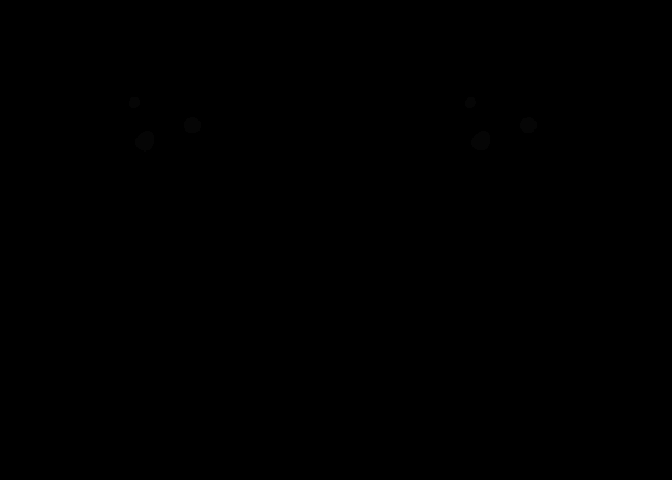
\includegraphics{tapas-vignette_files/figure-latex/unnamed-chunk-28-1.pdf}
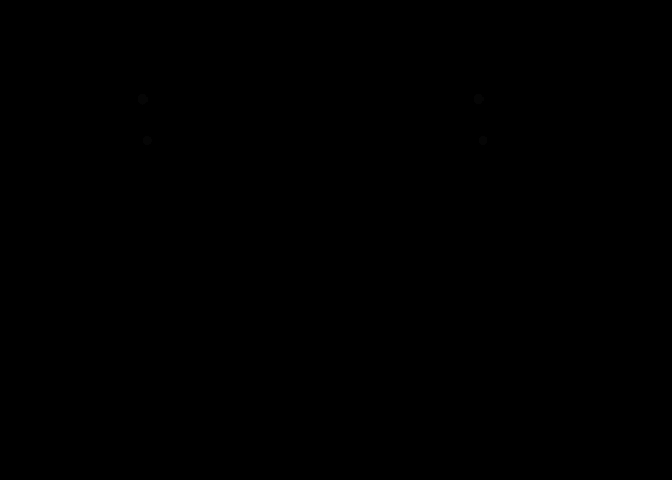
\includegraphics{tapas-vignette_files/figure-latex/unnamed-chunk-28-2.pdf}
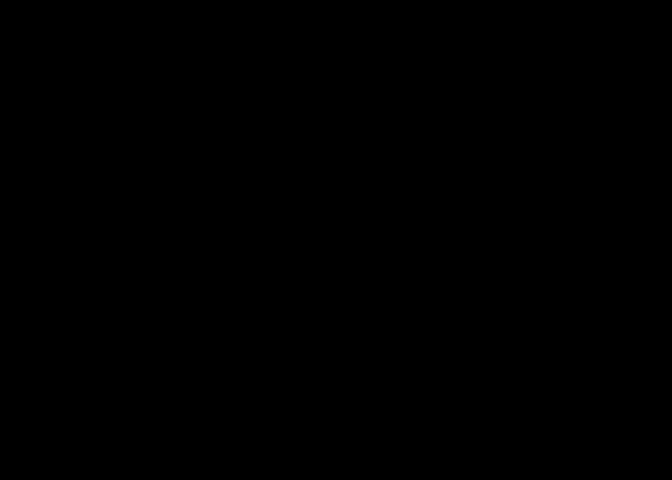
\includegraphics{tapas-vignette_files/figure-latex/unnamed-chunk-28-3.pdf}
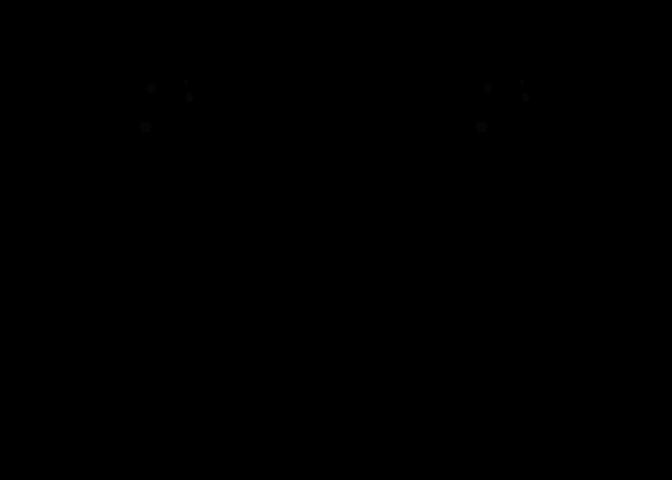
\includegraphics{tapas-vignette_files/figure-latex/unnamed-chunk-28-4.pdf}
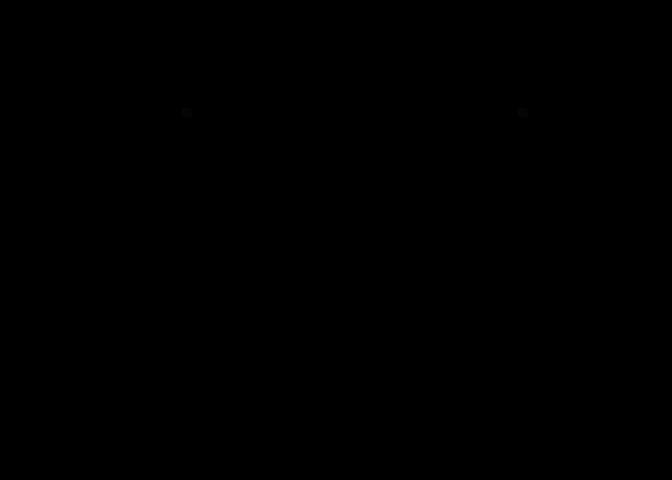
\includegraphics{tapas-vignette_files/figure-latex/unnamed-chunk-28-5.pdf}

\begin{verbatim}
#> integer(0)
\end{verbatim}

Now we will look at the group threshold produced binary segmentation
masks.

\begin{Shaded}
\begin{Highlighting}[]
\CommentTok{# The group threshold binary masks}
\NormalTok{oro.nifti}\OperatorTok{::}\KeywordTok{image}\NormalTok{(test_data1[[}\DecValTok{1}\NormalTok{]]}\OperatorTok{$}\NormalTok{group_binary_mask) }\OperatorTok{+}\StringTok{ }
\StringTok{  }\NormalTok{oro.nifti}\OperatorTok{::}\KeywordTok{image}\NormalTok{(test_data1[[}\DecValTok{2}\NormalTok{]]}\OperatorTok{$}\NormalTok{group_binary_mask) }\OperatorTok{+}
\StringTok{  }\NormalTok{oro.nifti}\OperatorTok{::}\KeywordTok{image}\NormalTok{(test_data1[[}\DecValTok{3}\NormalTok{]]}\OperatorTok{$}\NormalTok{group_binary_mask) }\OperatorTok{+}\StringTok{ }
\StringTok{  }\NormalTok{oro.nifti}\OperatorTok{::}\KeywordTok{image}\NormalTok{(test_data1[[}\DecValTok{4}\NormalTok{]]}\OperatorTok{$}\NormalTok{group_binary_mask) }\OperatorTok{+}
\StringTok{  }\NormalTok{oro.nifti}\OperatorTok{::}\KeywordTok{image}\NormalTok{(test_data1[[}\DecValTok{5}\NormalTok{]]}\OperatorTok{$}\NormalTok{group_binary_mask)}
\end{Highlighting}
\end{Shaded}

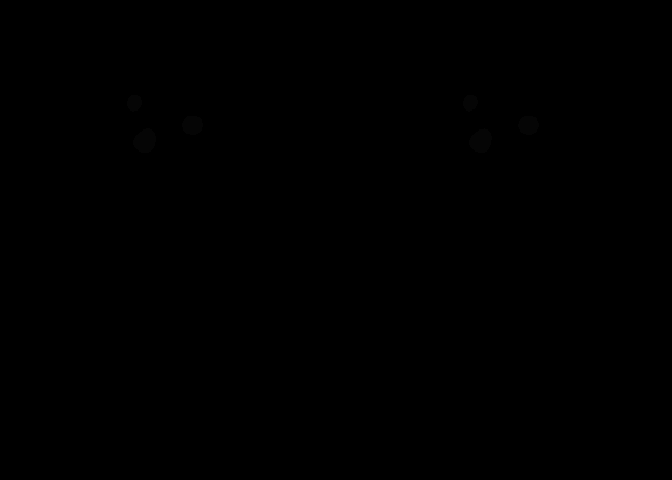
\includegraphics{tapas-vignette_files/figure-latex/unnamed-chunk-29-1.pdf}
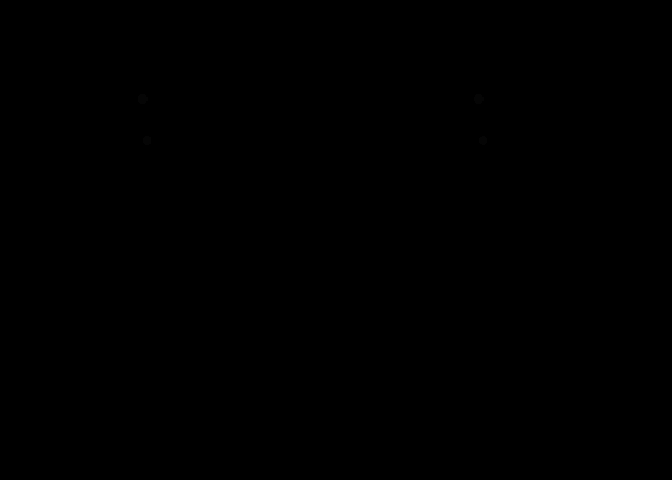
\includegraphics{tapas-vignette_files/figure-latex/unnamed-chunk-29-2.pdf}
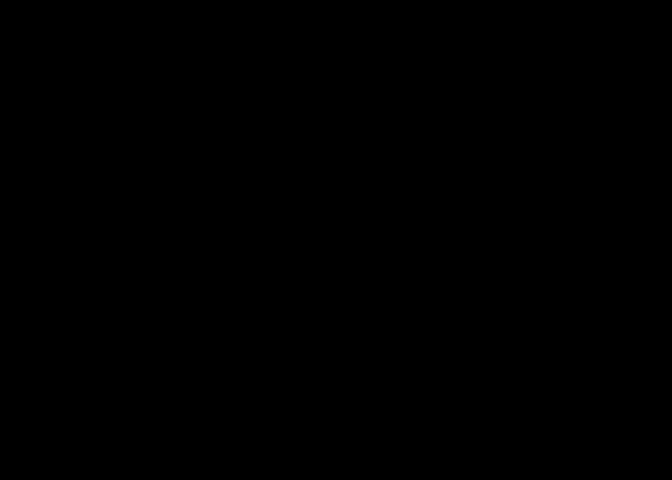
\includegraphics{tapas-vignette_files/figure-latex/unnamed-chunk-29-3.pdf}
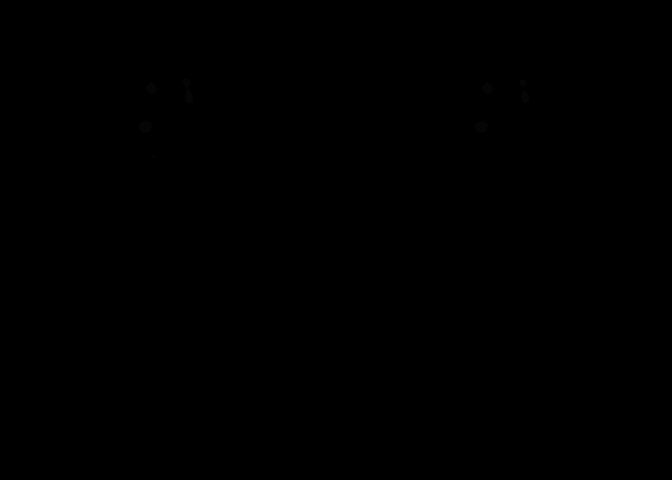
\includegraphics{tapas-vignette_files/figure-latex/unnamed-chunk-29-4.pdf}
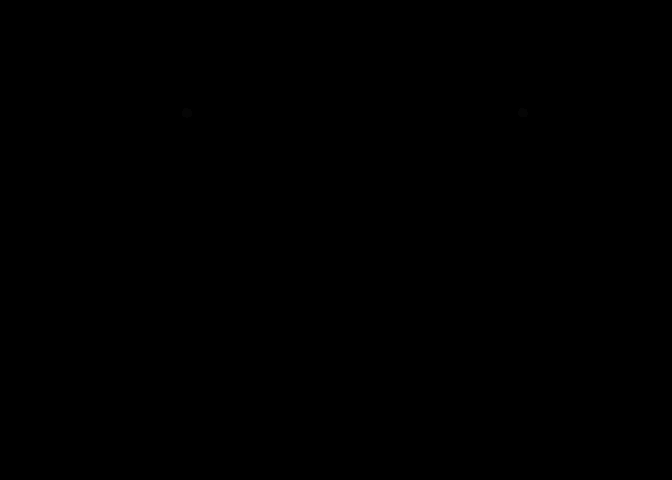
\includegraphics{tapas-vignette_files/figure-latex/unnamed-chunk-29-5.pdf}

\begin{verbatim}
#> integer(0)
\end{verbatim}

With these masks we can calculate DSC to compare the TAPAS and group
threshold masks.

\begin{Shaded}
\begin{Highlighting}[]
\CommentTok{# Calculate DSC in each mask}
\NormalTok{dsc =}\StringTok{ }\NormalTok{tibble}\OperatorTok{::}\KeywordTok{tibble}\NormalTok{(}
  \DataTypeTok{tapas_dsc =} \KeywordTok{c}\NormalTok{(aliviateR}\OperatorTok{::}\KeywordTok{dsc}\NormalTok{(test_gold_standard_masks[[}\DecValTok{1}\NormalTok{]], test_data1[[}\DecValTok{1}\NormalTok{]]}\OperatorTok{$}\NormalTok{tapas_binary_mask),}
\NormalTok{                aliviateR}\OperatorTok{::}\KeywordTok{dsc}\NormalTok{(test_gold_standard_masks[[}\DecValTok{2}\NormalTok{]], test_data1[[}\DecValTok{2}\NormalTok{]]}\OperatorTok{$}\NormalTok{tapas_binary_mask),}
\NormalTok{                aliviateR}\OperatorTok{::}\KeywordTok{dsc}\NormalTok{(test_gold_standard_masks[[}\DecValTok{3}\NormalTok{]], test_data1[[}\DecValTok{3}\NormalTok{]]}\OperatorTok{$}\NormalTok{tapas_binary_mask),}
\NormalTok{                aliviateR}\OperatorTok{::}\KeywordTok{dsc}\NormalTok{(test_gold_standard_masks[[}\DecValTok{4}\NormalTok{]], test_data1[[}\DecValTok{4}\NormalTok{]]}\OperatorTok{$}\NormalTok{tapas_binary_mask),}
\NormalTok{                aliviateR}\OperatorTok{::}\KeywordTok{dsc}\NormalTok{(test_gold_standard_masks[[}\DecValTok{5}\NormalTok{]], test_data1[[}\DecValTok{5}\NormalTok{]]}\OperatorTok{$}\NormalTok{tapas_binary_mask)),}
  \DataTypeTok{group_dsc =} \KeywordTok{c}\NormalTok{(aliviateR}\OperatorTok{::}\KeywordTok{dsc}\NormalTok{(test_gold_standard_masks[[}\DecValTok{1}\NormalTok{]], test_data1[[}\DecValTok{1}\NormalTok{]]}\OperatorTok{$}\NormalTok{group_binary_mask),}
\NormalTok{                aliviateR}\OperatorTok{::}\KeywordTok{dsc}\NormalTok{(test_gold_standard_masks[[}\DecValTok{2}\NormalTok{]], test_data1[[}\DecValTok{2}\NormalTok{]]}\OperatorTok{$}\NormalTok{group_binary_mask),}
\NormalTok{                aliviateR}\OperatorTok{::}\KeywordTok{dsc}\NormalTok{(test_gold_standard_masks[[}\DecValTok{3}\NormalTok{]], test_data1[[}\DecValTok{3}\NormalTok{]]}\OperatorTok{$}\NormalTok{group_binary_mask),}
\NormalTok{                aliviateR}\OperatorTok{::}\KeywordTok{dsc}\NormalTok{(test_gold_standard_masks[[}\DecValTok{4}\NormalTok{]], test_data1[[}\DecValTok{4}\NormalTok{]]}\OperatorTok{$}\NormalTok{group_binary_mask),}
\NormalTok{                aliviateR}\OperatorTok{::}\KeywordTok{dsc}\NormalTok{(test_gold_standard_masks[[}\DecValTok{5}\NormalTok{]], test_data1[[}\DecValTok{5}\NormalTok{]]}\OperatorTok{$}\NormalTok{group_binary_mask)))}
\CommentTok{# Print DSC}
\NormalTok{dsc}
\CommentTok{#> # A tibble: 5 x 2}
\CommentTok{#>   tapas_dsc group_dsc}
\CommentTok{#>       <dbl>     <dbl>}
\CommentTok{#> 1     0.528     0.424}
\CommentTok{#> 2     0.518     0.515}
\CommentTok{#> 3     0         0    }
\CommentTok{#> 4     0.502     0.469}
\CommentTok{#> 5     0.408     0.410}
\end{Highlighting}
\end{Shaded}

\hypertarget{thank-you}{%
\section{Thank you}\label{thank-you}}

Thank you all for the time and I hope you enjoyed the training vignette.
If you have comments, questions, or suggestions please feel free to
contact me by submitting an issue.

\begin{Shaded}
\begin{Highlighting}[]
\NormalTok{knitr}\OperatorTok{::}\KeywordTok{include_graphics}\NormalTok{(}\StringTok{"../inst/end.jpg"}\NormalTok{)}
\end{Highlighting}
\end{Shaded}

\begin{center}
\includegraphics[width=8.33in]{../inst/end} \end{center}

\begin{Shaded}
\begin{Highlighting}[]
\CommentTok{# Run this in console. Knit does not work properly. Saves to wrong directory}
\NormalTok{rmarkdown}\OperatorTok{::}\KeywordTok{render}\NormalTok{(}\StringTok{"vignettes/tapas-vignette.Rmd"}\NormalTok{,}
                  \KeywordTok{c}\NormalTok{(}\StringTok{"html_vignette"}\NormalTok{, }
                    \StringTok{"pdf_document"}\NormalTok{, }
                    \StringTok{"github_document"}\NormalTok{))}
\end{Highlighting}
\end{Shaded}


\end{document}
